\chapter{Design iteration II}
\label{DesignIteration2}
\begin{flushright}{\slshape    
If interaction design is considered only at the end, \\
software is driven by engineering design, of which \\
users are rightly unaware, rather than by representations \\
with which they interact.} \\ \medskip
    --- Gillian Crampton Smith and Philip Tabor \cite{Winograd1996}
\end{flushright}

\marginpar{Parts of this chapter appear in \cite{Niezen2011}, \cite{Vlist2011} and \cite{VanderVlist2012a}.}

The second iteration was driven by a collaboration with various partners in the \ac{SOFIA} project, which included Philips, NXP, Conante and the TU/e \ac{SAN} research group. This collaboration culminated in a joint demonstrator that was exhibited and evaluated at the Experience Lab at the High Tech Campus in Eindhoven --- the Smart Home pilot.

The goals of the Smart Home pilot were as follows:

\begin{itemize}
	\item Conduct a pilot study with users in a setting that resembles a real home
	\item Demonstrate the system to stakeholders and other interested parties
	\item Serve as a feasibility study
	\item Test how stable the implementation would be when it would be running for a full week
	\item Serve as an experimental setup for user experiments
\end{itemize}

More general goals of this design iteration were to improve our approach to solve interoperability problems between devices using semantic technologies, and to test our approach to technology integration with an increased number of devices.

\section{Requirements}
\label{D2Requirements}
%- Should allow for actively or automatically manipulable instances (Semantic transformers?) \cite{Mitsui08}

The Smart Home pilot is based on the following scenario:

\textit{Mark and Dries enter their home. A presence sensor detects their presence and notifies the smart space. The decorative wall-wash lights are in turn notified of user presence by the smart space, and turn themselves on. Mark and Dries start listening to music. They would like to try to render the music on a lighting device to also create some visual effects accompanying the music. They query the smart space and find out that the lighting device can render these light effects. They make a connection between the music player and the lighting device using the Connector. The light starts being rendered on the lighting device. To put the focus on the lighting device, the decorative wall-wash lights in the room automatically dim themselves down. At the same time, the light pattern also starts being rendered on the remote lighting device, where Mark's sister Sofia can observe the same light effects in her own house.}

\textit{At another location: Sofia enters her house and the intelligent lighting system detects her presence, notifies the smart space and switches the lights on. After a while, Sofia is curious and wants to listen to the music that Mark and Dries are listening to. She connects her lighting device to her stereo using Spotlight Navigation, and the same song plays on her surround sound system.}

There are some obvious similarities with the previous scenario in Chapter \ref{DesignIteration1}. However, there are a number of additional devices introduced:

\begin{itemize}
	\item Presence sensor and wall-wash lighting - A system developed by TU/e \ac{SAN} that detects the user's presence and switches the lights on automatically
	\item Lighting device - An ambient lamp developed by Philips, based on their LivingColors technology
	\item Intelligent lighting system - A lighting system developed by NXP that also detects the presence of users
	\item Spotlight Navigation - An augmented reality approach to exploring semantic connections, based on technology developed by Conante
\end{itemize}

This increase in the heterogeneity of devices helps us to see if the ontology-based approach can be applied to a larger range of devices, and the increase in system complexity is used to test the capabilities of the software framework.
We first focus on the design of the ontologies that were created to support these kind of scenarios, followed by the design of the devices that were created specifically for the pilot.


\section{Ontology Design}
\label{OntologyDesign2}

The \emph{Semantic Media} ontology and \emph{Semantic Interaction} ontology were created during Iteration II to enable interoperability between the devices of the different partners involved in the Smart Home pilot.

\subsection{Semantic Media ontology}
\label{SemanticMediaOntology}

%begin S3E
% \begin{figure}
% \centering
% 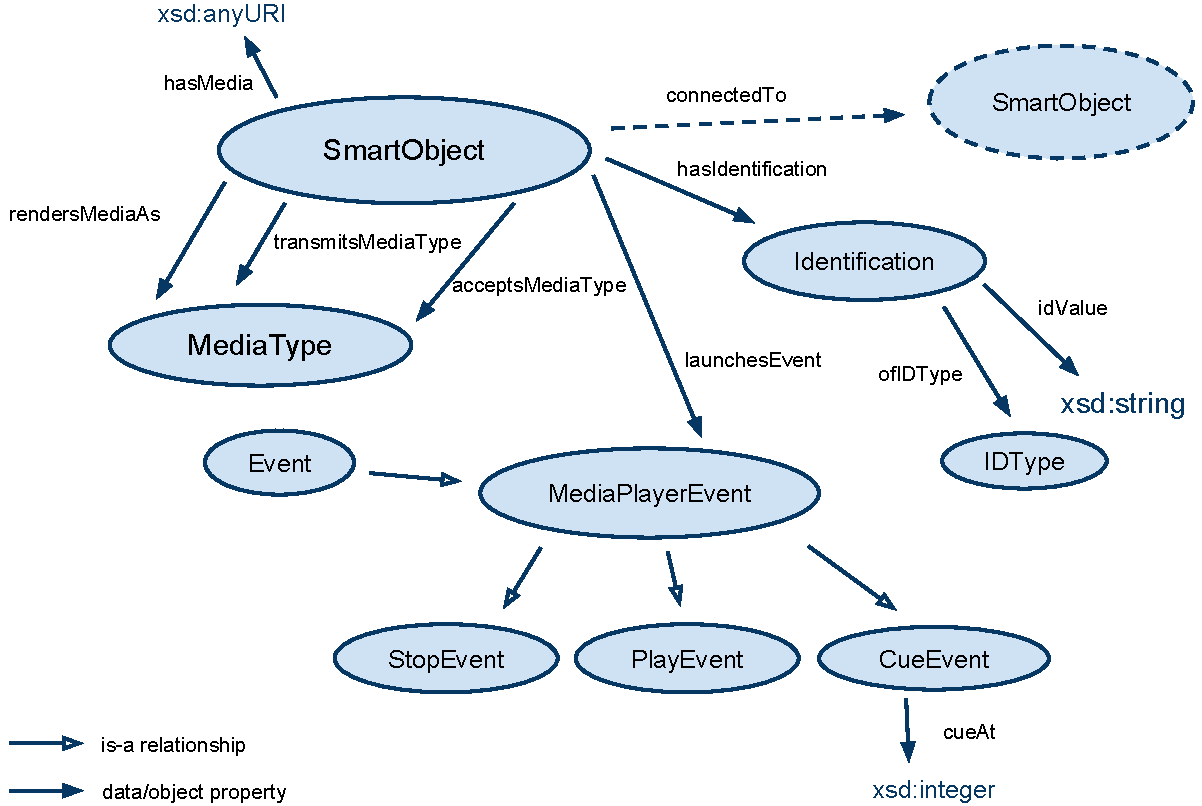
\includegraphics[width=300px]{SemanticMediaOntology}
% \caption{Semantic Media Ontology}
% \label{semanticMediaOntology}
% \end{figure}


\begin{figure}[bth]
	\digraph[scale=0.45]{ontologyInstance}{
		rankdir=LR;
		%node[shape="box"];
		anyURI [label="xsd:anyURI", shape="plaintext"];
		integer [label="xsd:integer", shape="plaintext"];
		datetime [label="xsd:datetime", shape="plaintext"];
		SmartObject -> MediaPlayerEvent [label="launchesEvent"];
		SmartObject -> MediaType [label="rendersMediaAs"];
		SmartObject -> MediaType [label="transmitsMediaType"];
		SmartObject -> MediaType [label="acceptsMediaType"];
		SmartObject -> anyURI [label="hasMedia"];
		MediaPlayerEvent -> StopEvent [style="dotted"];
		MediaPlayerEvent -> PlayEvent [style="dotted"];
		MediaPlayerEvent -> CueEvent [style="dotted"];
		CueEvent -> integer [label="cueAt"];
		Event -> MediaPlayerEvent [style="dotted"];
		Event -> datetime [label="inXSDDateTime"];
	}
	\caption{Semantic Media Ontology}
	\label{semanticMediaOntology}
\end{figure}\marginpar{The notation used for Figure \ref{semanticMediaOntology} was also used in Figure \ref{ontologyInstance} in Section \ref{OntologyDesign1}, where class membership is denoted with dotted lines and relationships are denoted with solid lines.}



The Semantic Media ontology, shown in Figure \ref{semanticMediaOntology}, is an application ontology that allows for describing media-specific device capabilities and related media content. A mobile device may be described as follows:


{\footnotesize
\begin{minted}{turtle}
MobileDevice rdf:type :SmartObject .
MobileDevice acceptsMediaType Audio .
MobileDevice transmitsMediaType Audio .
MobileDevice hasMedia "file://media/groove.mp3"^^xsd:anyURI .
MobileDevice rendersMediaAs Audio .
\end{minted}
}

The system configures itself through semantic reasoning based on these media type descriptions. \marginpar{An example of semantic reasoning with media type descriptions is described in Section \ref{D2Implementation}.} A media player event of type \texttt{PlayEvent}, that would be generated when the mobile device starts playing music, is described as follows:

{\footnotesize
\begin{minted}{turtle}
event1234-ABCD rdf:type PlayEvent .
event1234-ABCD inXSDDateTime "2001-10-26T21:32:52"^^xsd:dateTime .
MobileDevice launchesEvent event1234-ABCD .
\end{minted}
}

Smart objects may be connected to one another using the \texttt{connectedTo} relationship. When a device receives an event notification, it first verifies that it is currently connected to the device that generated the event, before responding to the event.

Smart objects may be connected to one another directly if there is a semantic match between transmitted and accepted media types. Otherwise a \emph{semantic transformer} will have to be be introduced to transform the shared content, while still preserving the actual meaning of the connection. \marginpar{An example of a semantic transformer is described in Section \ref{D2Implementation}.}

\begin{description}
	\item [Semantic transformer] A semantic transformer is defined as a service that transforms information shared between devices from one type to another, while preserving the meaning of the information.
\end{description}

The concept of a semantic transformers is considered an important part of the theory developed in this work, and its applicability to smart environments in general is discussed in Chapter \ref{SemanticConnectionsTheory}.



%begin africon
\subsection{Semantic Interaction ontology}
\label{sectionSemanticInteractionOntology}

% \begin{figure}
% \centering
% 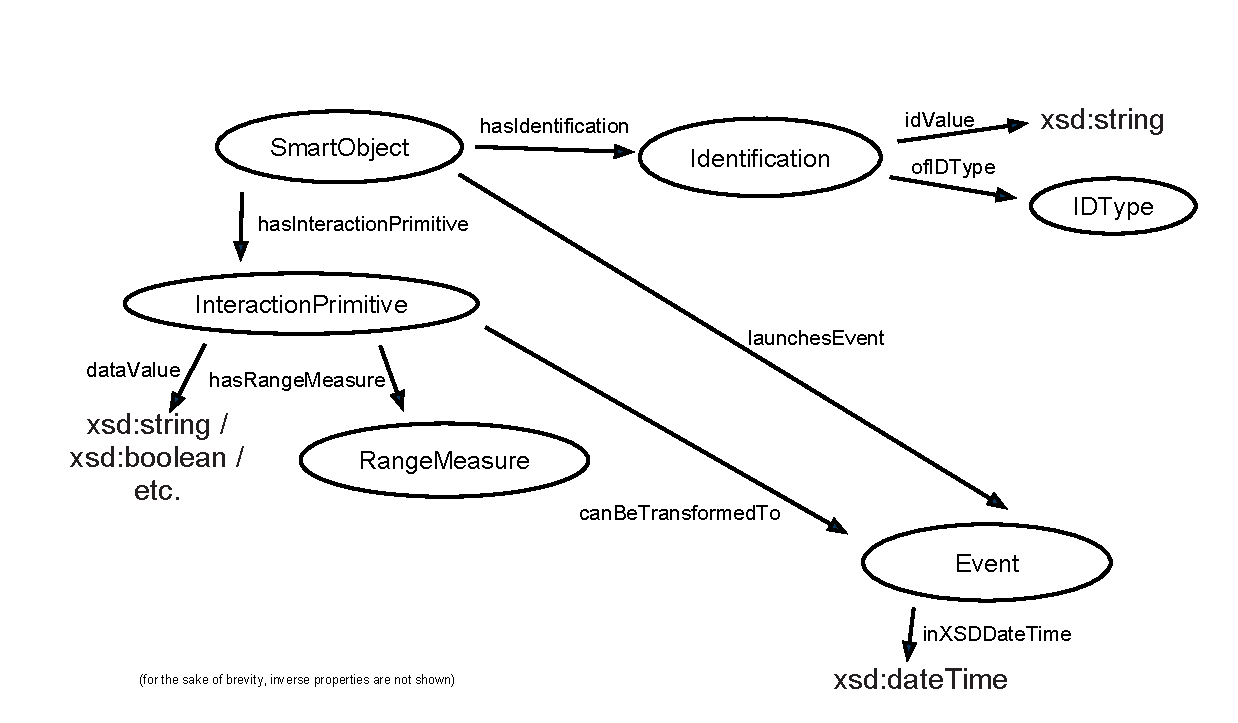
\includegraphics[width=350px]{SemanticInteractionOntology}
% \caption{Semantic Interaction Ontology}
% \label{semanticInteractionOntology}
% \end{figure} 


\begin{figure}[bth]
	\centerline{
	\digraph[scale=0.45]{ontologyInstance2}{
		rankdir=LR;
		%node[shape="box"];
		etc [label="xsd:string / xsd:boolean / etc.", shape="plaintext"];
		string [label="xsd:string", shape="plaintext"];
		SmartObject -> InteractionPrimitive [label="hasInteractionPrimitive"];
		SmartObject -> Event [label="launchesEvent"];
		InteractionPrimitive -> etc [label="dataValue"];
		InteractionPrimitive -> RangeMeasure [label="hasRangeMeasure"];
		InteractionPrimitive -> Event [label="canBeTransformedTo"];
		SmartObject -> Identification [label="hasIdentification"];
		Identification -> string [label="idValue"];
		Identification -> IDType [label="ofIDType"];
	}}
	\caption{Semantic Interaction Ontology}
	\label{semanticInteractionOntology}
\end{figure}


The Semantic Interaction ontology we have developed is shown in Figure \ref{semanticInteractionOntology}.  A device, defined as a \texttt{SmartObject}, is uniquely identified by some kind of \texttt{Identification}, for example a IP address and port number, \ac{RFID} tag or barcode. \marginpar{Identification is discussed in Section \ref{Identification}.} Different ID types can be defined as required. Devices can then launch events, for example a media player can generate a \texttt{PlayEvent} when music starts playing.


A smart object is described in terms of its \emph{interaction primitives}. This new concept, as well as the other new concepts introduced in this section, refine the ontology that was introduced in the first design iteration:


\begin{description}
	\item [Interaction primitive]An \emph{interaction primitive} is defined to be the smallest addressable element that has a meaningful relation to the interaction itself. 
\end{description}

\marginpar{The concept of interaction primitives is discussed in more detail in Section \ref{InteractionPrimitives}.}
As an example of how the ontology may be used, we start off by defining a smart object and its interaction primitives. Recall that it is only necessary to describe interaction primitives of a device if we use that device's interaction primitive to control another device through the smart space. We can, for example, describe the volume control rocker switch on a smart phone as an interaction primitive:

\begin{minted}{turtle}
SmartPhone rdf:type SmartObject .
PhoneRockerSwitch rdf:type InteractionPrimitive .
SmartPhone hasInteractionPrimitive PhoneRockerSwitch .
\end{minted}

We now need to define the properties of the interaction primitive. We start by describing the range measure, or the range of values that the interaction primitive can produce (e.g. the rocker switch can produce \texttt{Up}, \texttt{Down} or \texttt{Neutral} values).

The range of values that an interaction primitive can take on is specified using a \texttt{RangeMeasure}.  These range measures are similar to the measure of the domain set used by MacKinlay et al \cite{MacKinlay1990}.\marginpar{MacKinlay's work was discussed in Section \ref{interactionTasks}.} Using the range measures, we can then infer which transformations may be used to map the input values to other interaction primitives or events. The ontology could be extended to also describe the different manipulation operators of the interaction primitive, e.g. rotation on the z-axis or movement along the y-axis. Note that the model of MacKinlay et al. has only been applied to \acp{GUI}. Similar models for ubiquitous computing have so far not given comprehensive taxonomies of input devices. Our approach of using interaction primitives to describe input devices is an attempt at providing such a taxonomy.

%The list of range measures is shown in Table \ref{rangeMeasures}.
% \begin{table}
%     \myfloatalign
%   \begin{tabularx}{\textwidth}{Xl} 
% 	\toprule
%     \tableheadline{Range measure} & \tableheadline{Possible values} \\ 
%     \midrule
% 
% 	Binary & True/False, 0 or 1 \\
% 	SingleDigit & up to 9 discrete values \\
% 	DoubleDigit & up to 99 discrete values \\
% 	TripleDigit & up to 999 discrete values \\
% 	LargeDigit & more than 1000 discrete values\\
% 	
%     \bottomrule
%   \end{tabularx}
%   \caption{Range measures for interaction primitives}\label{rangeMeasures}
% \end{table}

% In our example we specify the \texttt{RangeMeasure} of our interaction primitive as follows:
% 
% \begin{minted}{turtle}
% PhoneRockerSwitch hasRangeMeasure SingleDigit
% \end{minted}


The actual data value of the interaction primitive is described using the \texttt{dataValue} property. Data values may be strings, boolean values or other datatypes, e.g.:

\begin{minted}{turtle}
PhoneRockerSwitch dataValue "neutral"^^xsd:string .
\end{minted}

When \texttt{PhoneRockerSwitch} is pressed, the data value is updated with:

\begin{minted}{turtle}
PhoneRockerSwitch dataValue "up"^^xsd:string .
\end{minted}

This enables other devices to make use of the user input on the \texttt{PhoneRockerSwitch}, irrespective of the interaction events generated. In fact, using \texttt{Transformation}, it becomes possible to map the physical, generic button presses from interaction primitives like \texttt{Phone\-Rocker\-Switch} to specific high-level events like \texttt{VolumeUpEvent} or
\texttt{Volume\-Down\-Event} using the default transformation \texttt{AdjustLevel} as is described in Table \ref{transformationTable}.

By specifying the transformation using the proper \ac{OWL} 2 semantics, the reasoner should be able to infer which user inputs can be mapped to which specific high-level events. This shows up as a \texttt{canBeTransformedTo} property between an interaction primitive and an event. In our example, this means that the following relationship will be inferred:

\begin{minted}{turtle}
PhoneRockerSwitch canBeTransformedTo VolumeEvent .
\end{minted}

\noindent
where the \texttt{"up"} data value may then be mapped to \texttt{Volume\-Up\-Event} and the \texttt{"down"} may be mapped to \texttt{VolumeDownEvent}, which are both sub-classed from \texttt{VolumeEvent}. This prevents situations where arbitrary mappings causes some of the semantics of the interaction to disappear.


\section{Device Design}

In the Smart Home pilot, the partners involved each created their own device or system to showcase the work they have performed during the \ac{SOFIA} project. The interoperability of the system architecture was tested and demonstrated by having these devices working together, even though they were created by different manufacturers at different times. We now describe these devices in more detail.

\subsection{Wall-wash lighting and presence sensors}

\begin{figure}
\centering
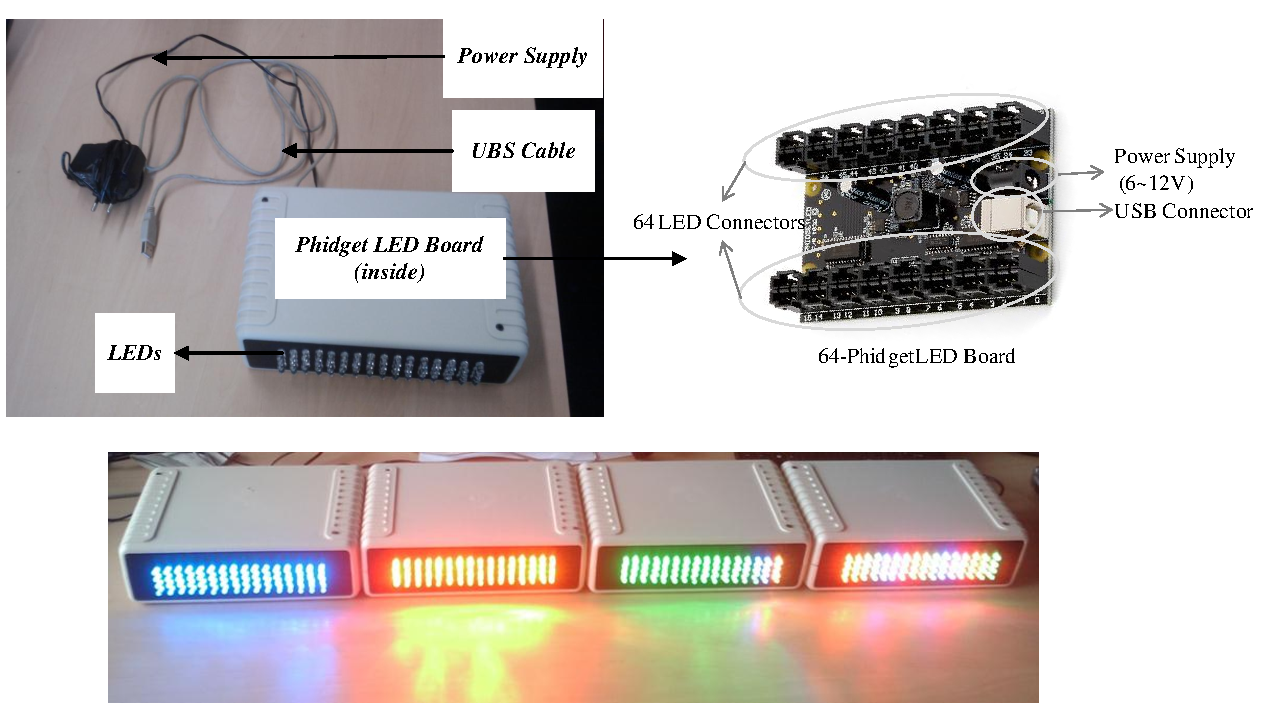
\includegraphics[width=250px]{lamp-KP}
\caption{Wall-wash lighting developed by TU/e SAN}
\label{wallwash}
\end{figure}

The decorative wall-wash lights consisted of four LED lamps, custom-built by the TU/e \ac{SAN} group, capable of generating coloured illumination on the wall of the room. The lamps are shown in Figure \ref{wallwash}, including a description of its components. A presence sensor determines the presence of a user in a designated area of the room and sends the presence information to the \ac{SIB}. The wall-wash lighting \ac{KP} is subscribed to this presence information, and its state is modified based on this information. There are two states updated on the \ac{SIB}: \texttt{Away} and \texttt{Present}. For example, when the \texttt{Present} state is specified, the Lamp \ac{KP} sends  the \texttt{ON} command to the wall-wash lighting, and the \texttt{OFF} command when the \texttt{Away} state is specified.  


\subsection{Connector object}
\label{Connector}
This device builds on the work done in the previous iteration by exploring another tangible approach for manipulating semantic connections. While devices are still identified with \ac{RFID} tags, the device itself is now mobile, and makes use of more meaningful interactions and feedback to establish and break connections.

\begin{figure}
\centering
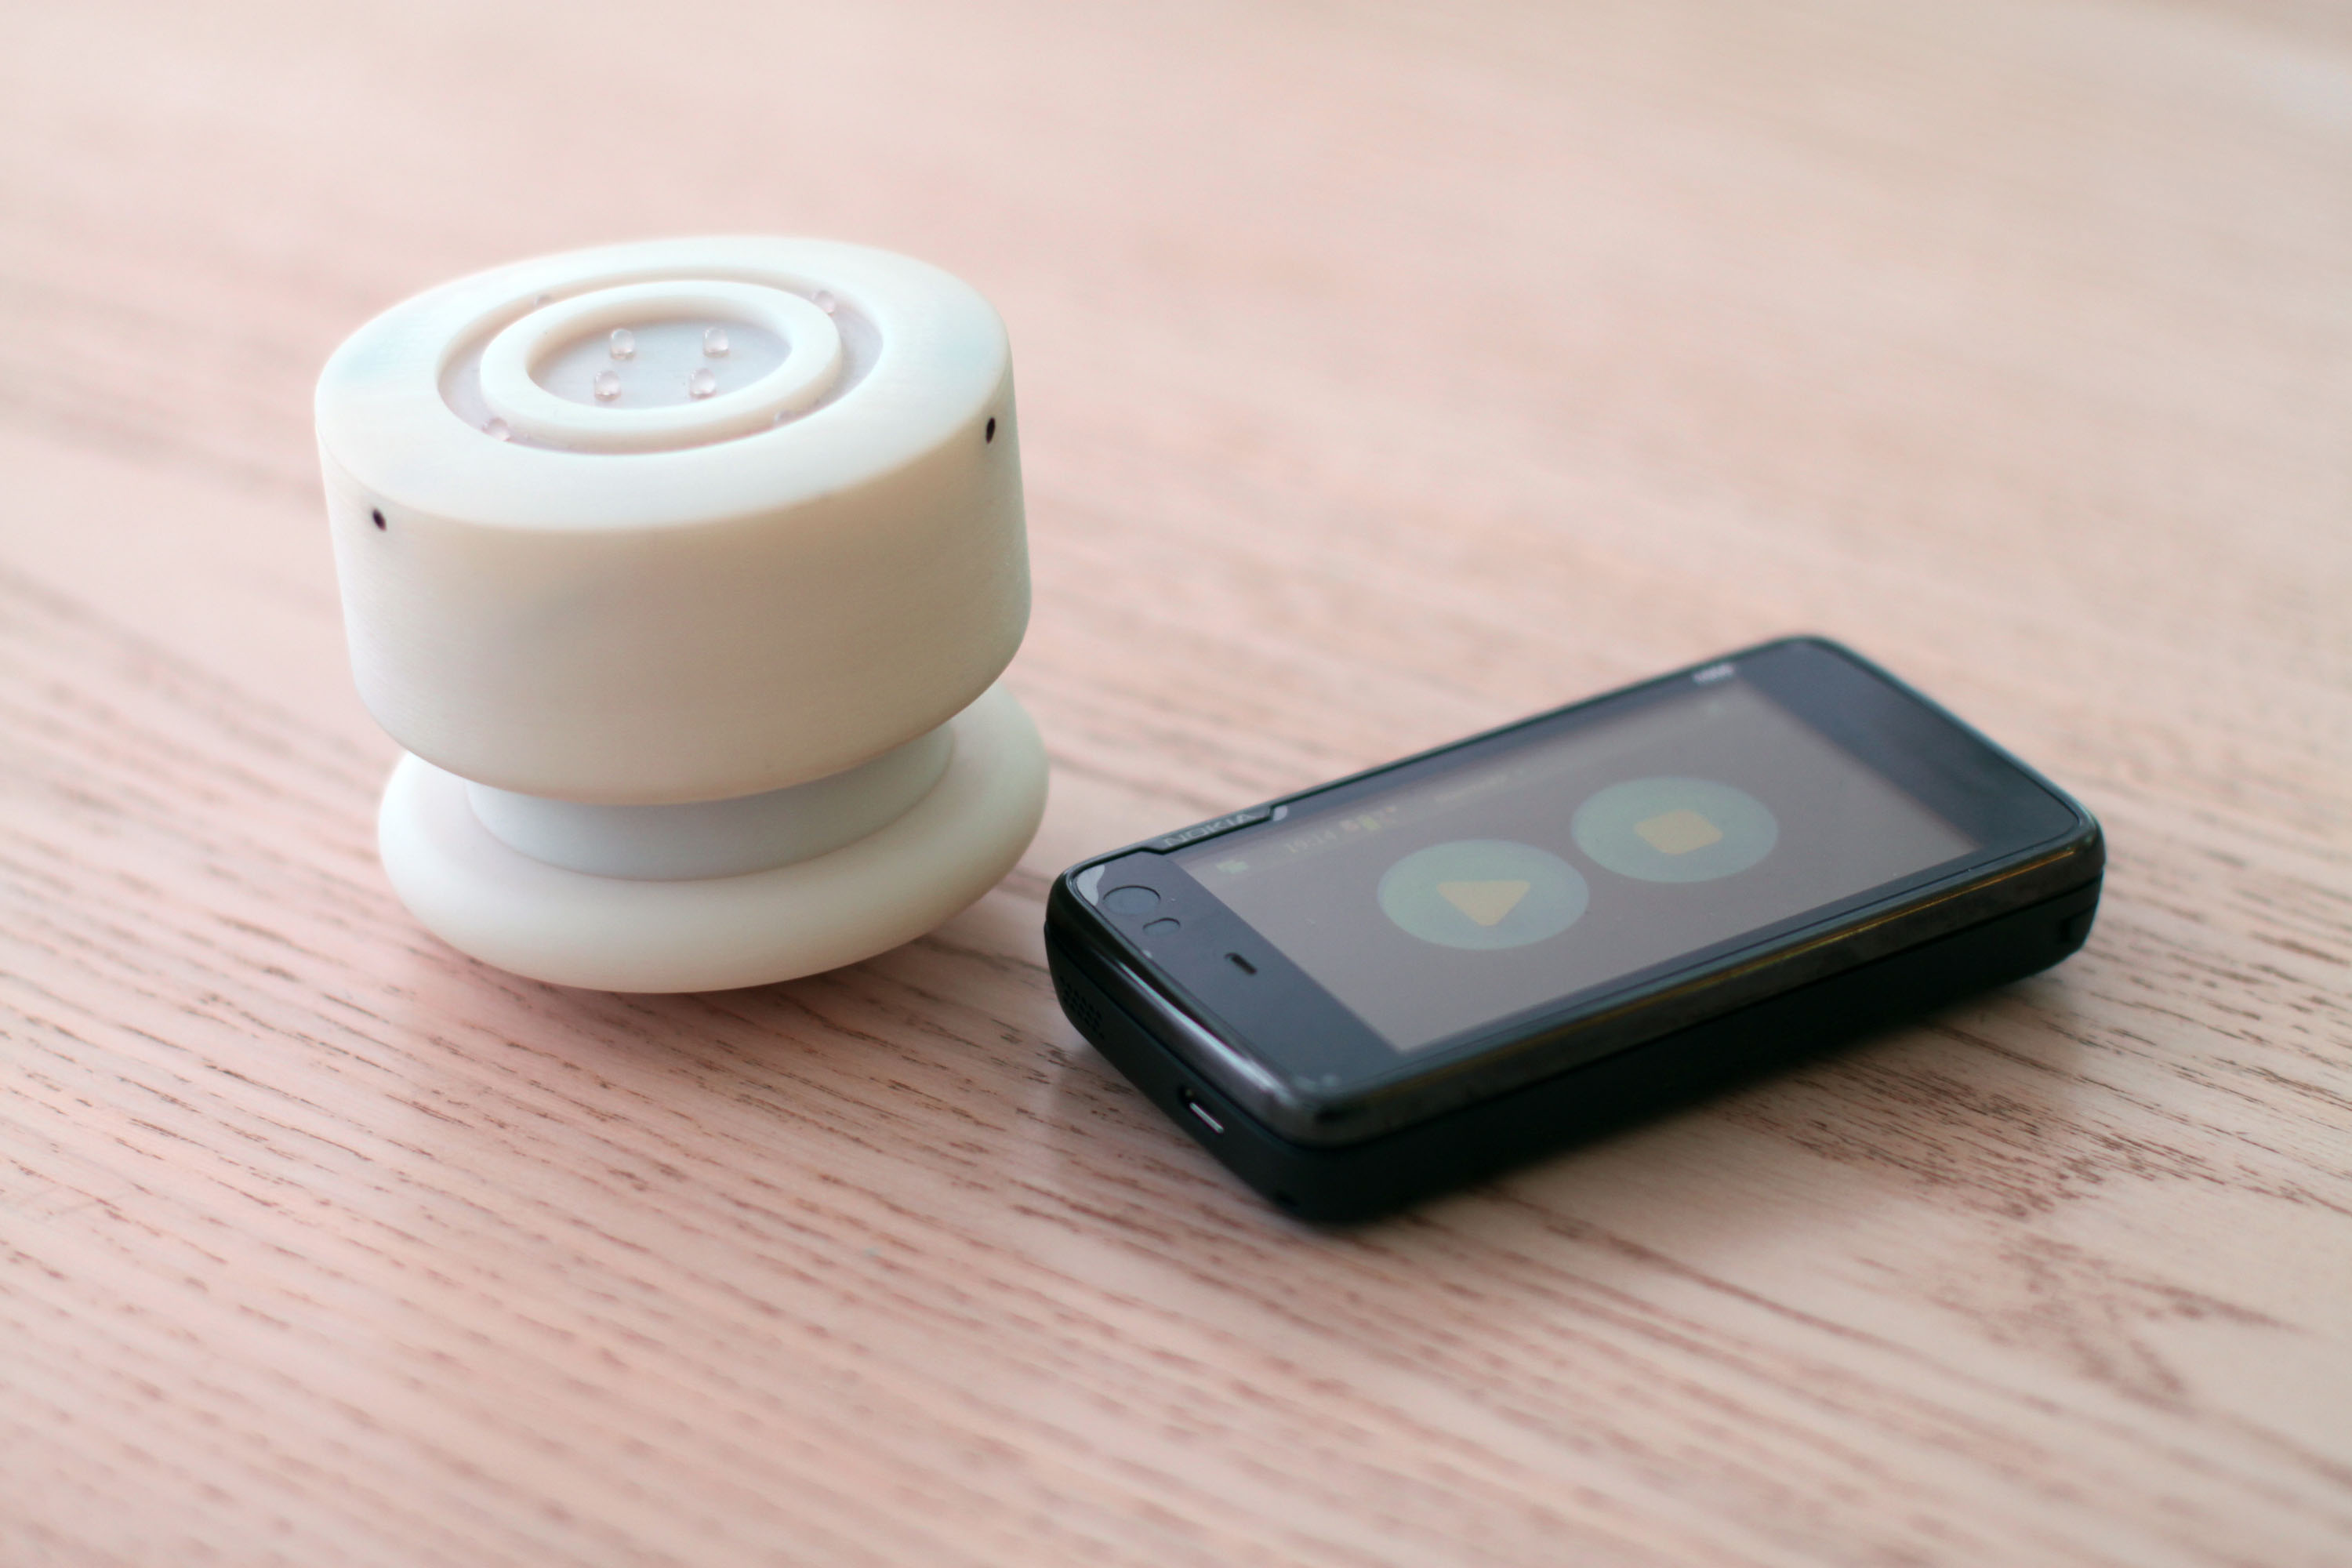
\includegraphics[width=300pt]{connector}
\caption{The Connector prototype and a smart phone used as a media player}
\label{connector}
\end{figure}

The Connector object, shown in Figure \ref{connector}, can be used to explore and manipulate semantic connections between different devices in the home environment. It is a handheld device that identifies devices, by scanning \ac{RFID} tags that are located on the devices themselves. By holding the Connector on top of the tag, users can explore the connection possibilities that are visualised with lights on top of the Connector. After holding the device in the \ac{RFID} field for a moment, the device-ID is locked and the other device to be connected can be selected in a similar fashion. With a push-to-click action a connection between two devices can be established. For removing an existing connection, the ring on the lower part of the device should be pulled until it clicks.

The cylindrical shape of the Connector is loosely inspired by that of a loupe or hand lens. By moving the connector over a tag, the connection possibilities can be ``read'' from the top of the cylinder. The display consists of two rings (made up of LEDs), each divided into 4 segments. The Connector supports several actions:

\begin{itemize}
	\item Explore - You can move it over an object or tag to see whether it is active.
	\item Select - A device or object can be selected by holding the connector close to or on a tag until the selection sequence is completed.
	\item Connect/disconnect - The connector can be compressed by pushing the top and the lower part together (connect), and it can be pulled, by pulling the lower part and the top part away from one another until it clicks (disconnect).
\end{itemize}   

When the tag is in the range of the Connector's \ac{RFID} field, it reads the tag and the first (yellow) light segment on top of the Connector will light up, serving as feedback that the Connector recognises the device. After holding the Connector over a device tag for a moment, a sequence starts, lighting up the second, third and fourth segment of the inner ring. After the device is recognised and selected, another device may be selected in a similar fashion. Now, the second ring of lights will start lighting up in sequence and one should wait until both rings are fully lit. Removing the Connector from the tag prematurely cancels the selection process.

When a connection between the selected devices is possible, both rings start flashing green. When no connection is possible, they will turn red. When a connection between the devices you scanned already exists, the rings will turn green. To make the connection, the Connector is compressed by pushing the top and lower part together, or by pushing the Connector down on the device it is touching, until it clicks. To remove an existing connection between two scanned devices, the ring on the lower part of the Connector should be pulled until it clicks. The rings will show a red light to indicate that the connection has been broken. The segments will turn off once the Connector is moved away from the device. Performing the opposite action of what is required to make or break a connection, cancels the procedure.

The Connector contains the following main components:

\begin{itemize}
\item Arduino Stamp 02
\item Innovations ID-12 125kHz RFID reader
\item SparkFun Bluetooth Mate Gold
\item 8 bi-colour LEDs
\item Switches
\item 3.3v LiPo battery (850 mAh)
\end{itemize}

In the previous iteration we had an issue with multiple tags within range of the reader at the same time, necessitating the use of 13.56MHz tags. Since only one tag is now read at a time we do not have this issue anymore, and as such 125KHz tags could be used. The Connector prototype is made out of four separate pieces which are 3D printed. The lower part and the top part of the Connector can be moved inward and outward serving as a two-way spring-loaded switch. The prototype packages all the necessary components into one integrated device which is wirelessly connected to a computer using a Bluetooth connection. 


\subsection{Spotlight Navigation}\label{SpotlightNavigation}

\begin{figure}
\centering
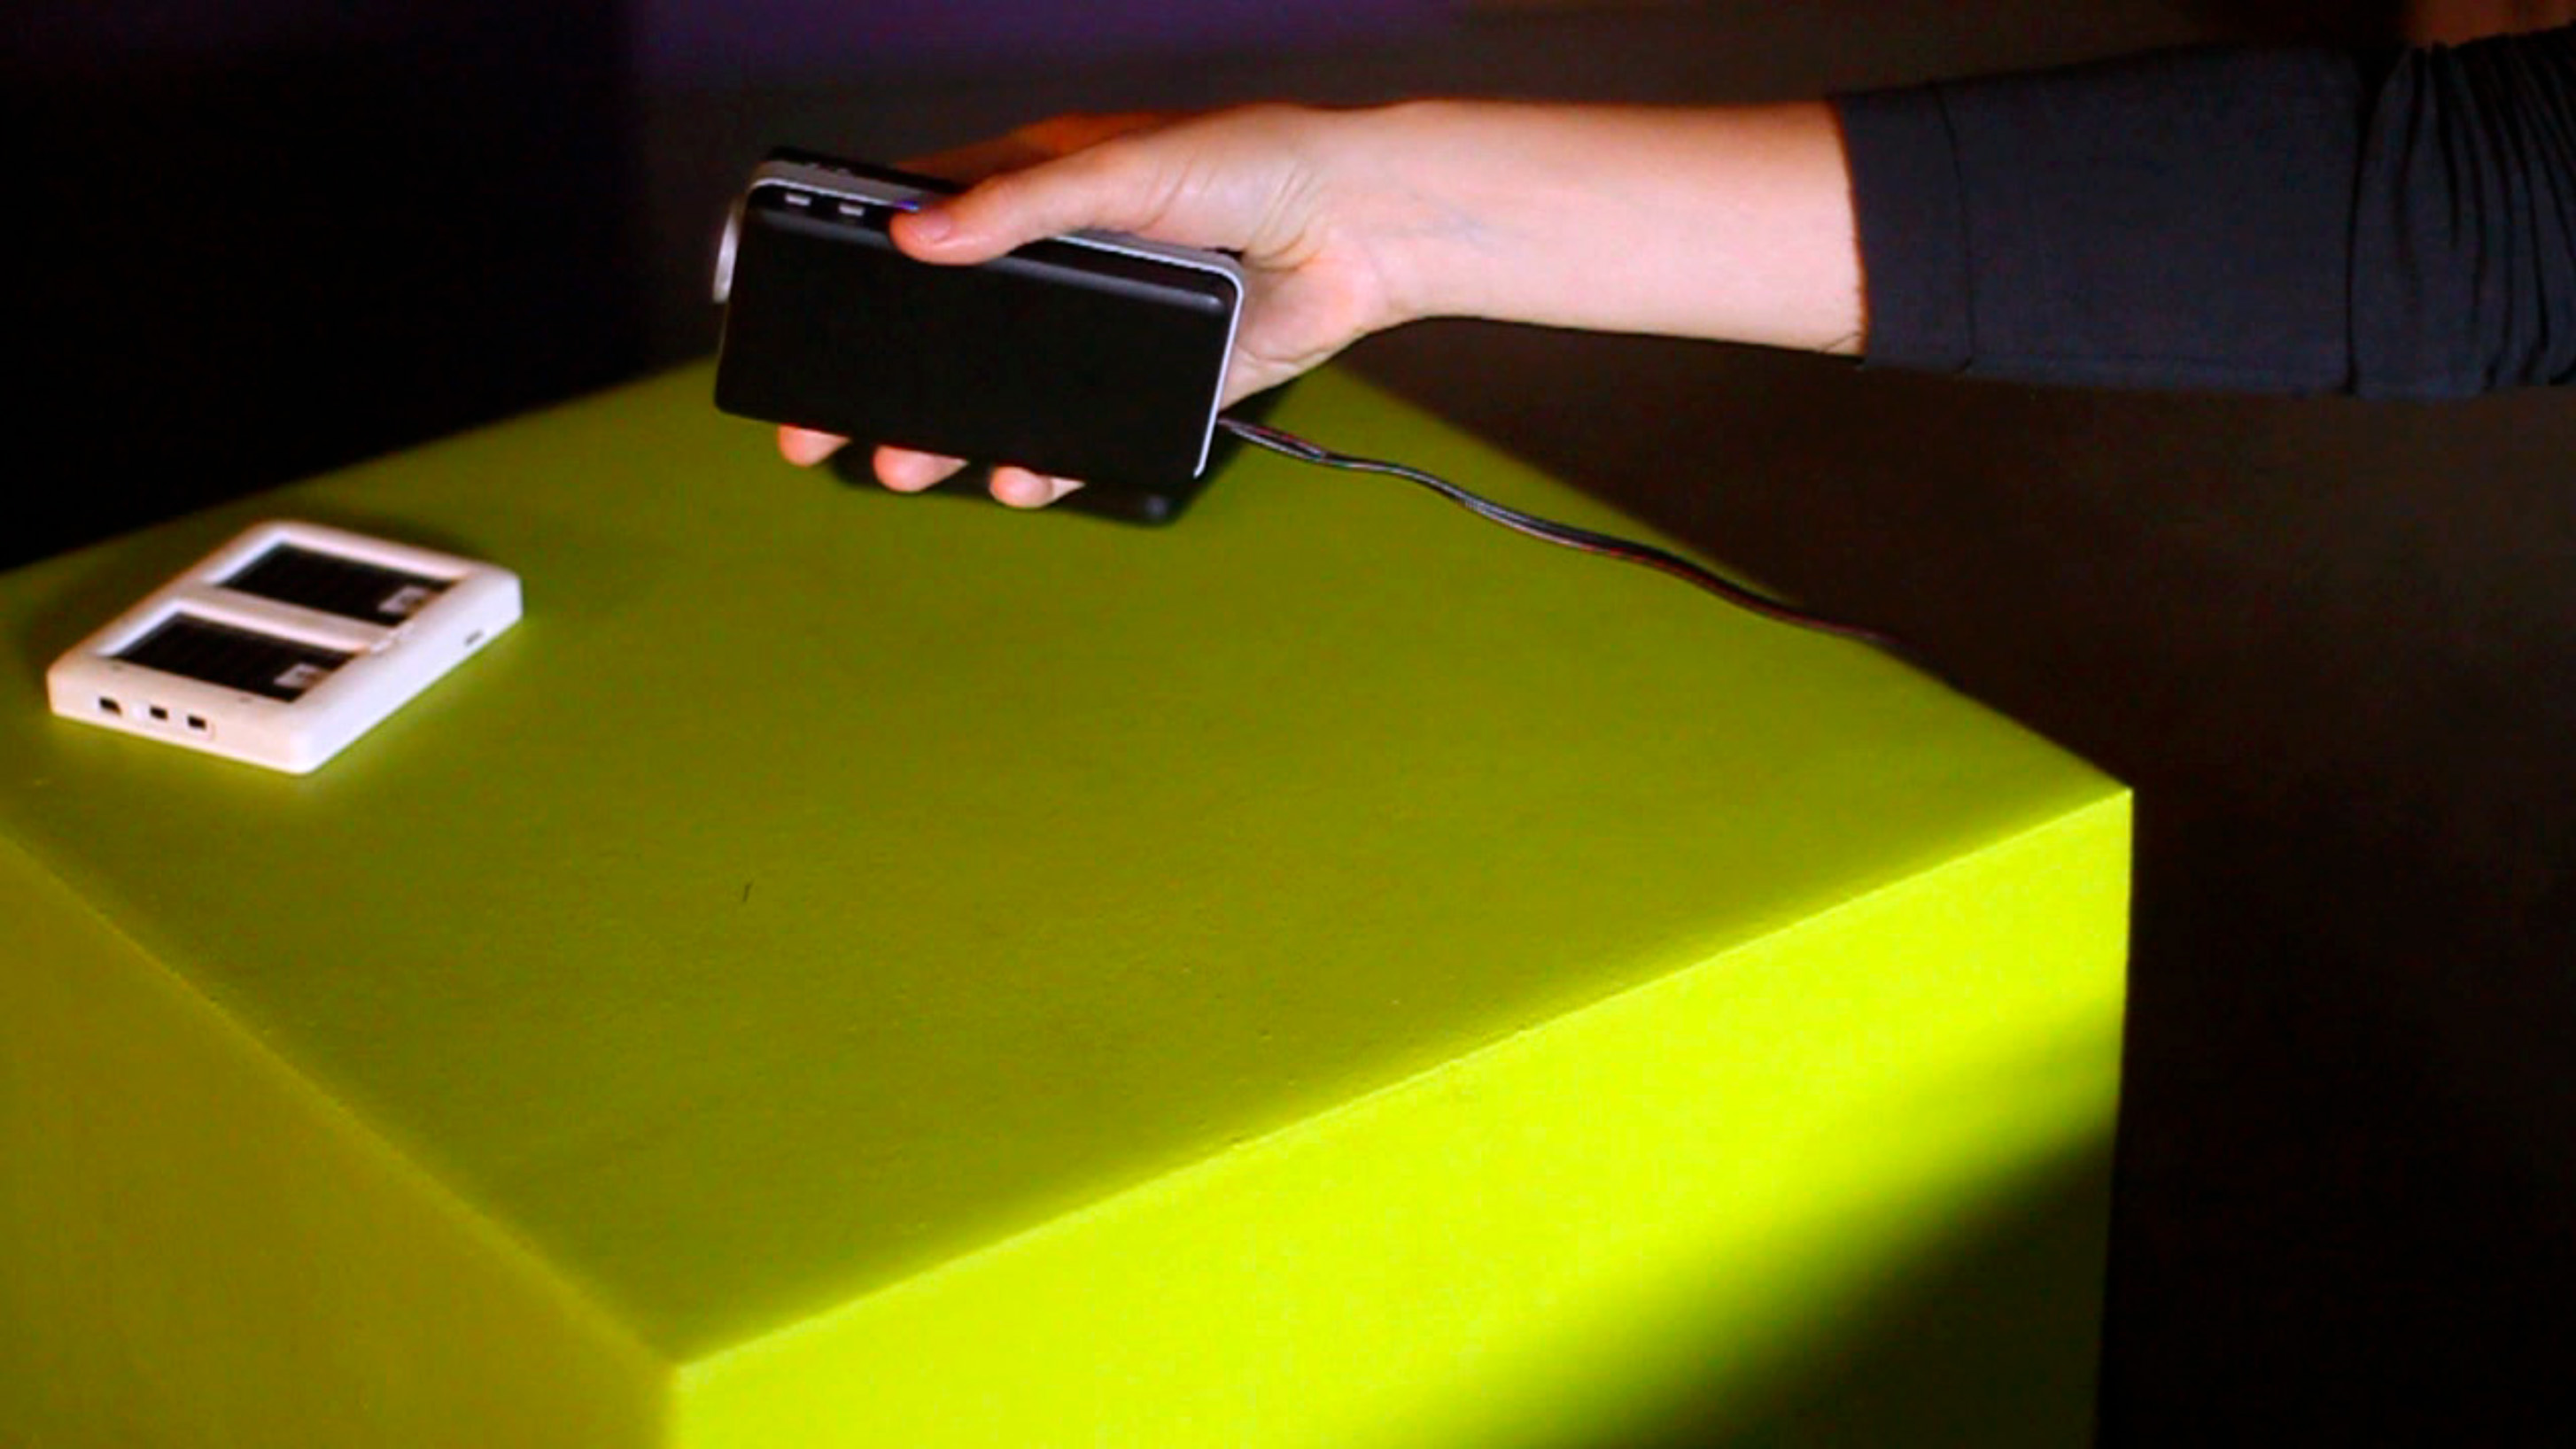
\includegraphics[width=300pt]{spotlightHand}
\caption{Spotlight Navigation prototype}
\label{projector}
\end{figure}

The Spotlight Navigation device, designed by Conante and shown in Figure \ref{projector}, is another approach to explore and manipulate connections between smart devices. With Spotlight Navigation, connection information contained in the smart space is projected into the real world, augmenting the real environment with virtual information, making it intuitively perceivable for users. Spotlight Navigation projects icons close to the actual devices in physical space. It allows for the creation of new connections simply by drawing lines between these icons, using a ``pick-and-drop'' action with a push-button on the prototype (press and hold the button when pointing at one device, move over the second device and release the button). Additionally the connection possibilities are projected between devices that allow for a connection, by changing the colour of the projected line (while the connection is being drawn) from yellow to green when the line's end is moved over the frame of the targeted device. When a connection is impossible, the connecting line will turn red and disappears as soon as the button is released.

Spotlight Navigation was invented as an intuitive way of accessing large data spaces through handheld digital projection devices \cite{Rapp2010,VanderVlist2012a}. Rather than directly projecting the equivalent of a small LCD display, Spotlight Navigation continuously projects a small portion of a much larger virtual pane or data space. It is the device's orientation that defines which part of the larger pane is selected for display. This is done in such a way that the virtual data appears to have a fixed location in the real world. By moving the projector's light spot over the wall, users make portions of the data space visible through intuitive, direct pointing gestures. This intuitiveness stems from the fact that the projected content always stays roughly at the same physical place, regardless of the orientation of the device. It becomes visible depending on whether it is in the projector's light cone or not. In other words, users have the impression that they are illuminating a part of a conceptually unbounded virtual data space, just as if they would be looking at hieroglyphs on a huge wall in a tomb with a flashlight. As people are familiar with operating flashlights, the operation needs no or little training. When accessing a data space with the device, users can zoom in and out of the data space by using a scroll wheel control, resulting in a pan-and-zoom user interface. To visualise the semantic connections in physical space, we rely on the symbolic meaning of colour, where green colour means ``proceed'' and red means the opposite. Using green, yellow and red lines we aim at referring to the ``existence'' of a connection, the ``possibility'' of a connection or to indicate that a connection is not possible. Figure \ref{projection} shows the projection when connecting two devices together.


\begin{figure}
\centering
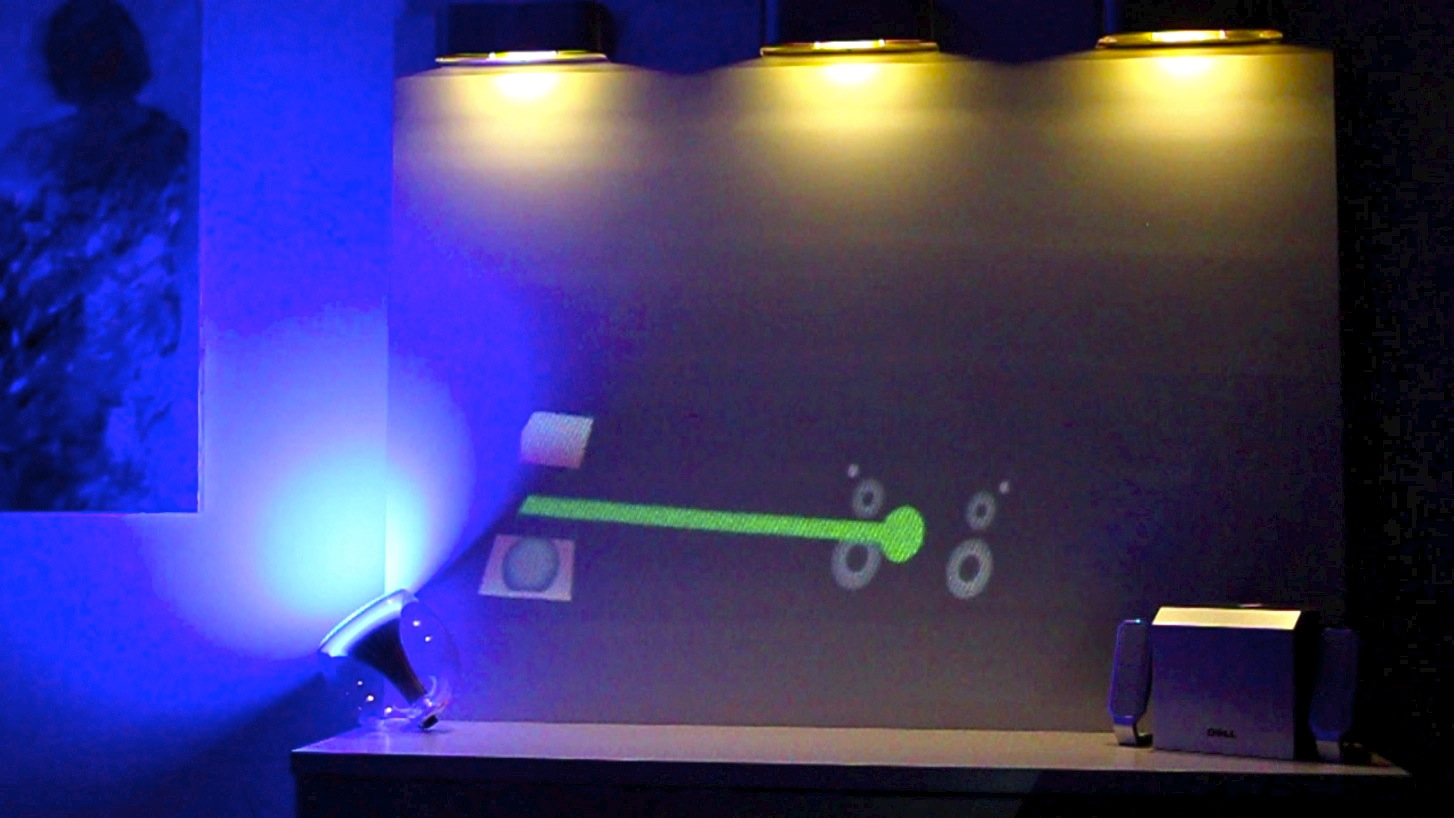
\includegraphics[width=300px]{projection}
\caption{Projection of the Spotlight Navigation when connecting two devices together}
\label{projection}
\end{figure}

With Spotlight Navigation, devices are identified by their physical location, relying strongly on \emph{natural mapping}. Connections are created simply by drawing lines between the devices. An erasing gesture with the Spotlight Navigation device pointed at an existing connection, breaks the connection. 

On a technical level, the operation is achieved through continuously measuring the orientation, and optionally also the position, of the device. Our prototype is using an inertial navigation module, also called an inertial measurement unit (IMU), that directly measure the orientation by means of accelerometers, gyroscopes and an electronic compass.

The Spotlight Navigation prototype is a fully embedded setup integrated into a 3D printed casing. The design of the casing was targeted at getting the smallest possible setup that could run on the integrated batteries. A dummy ring was added to the prototype to strengthen the semantics of a mobile projector. Figure \ref{projector} shows the prototype. Our current setup consists of the following components:

\begin{itemize}
\item OMAP3530 board (IGEP module)
\item Pico projector (Microvision SHOWWX)
\item Orientation sensor (Sparkfun 9DOF Razor IMU)
\item scroll wheel (with button press functionality)
\item two additional buttons
\item two 3.7v li-ion batteries (Nokia BL5J)
\end{itemize}

The OMAP3530 processor contains a 3D-graphics core (PowerVR) that is capable of
rendering the connection visualisations and device icons in real-time. The prototype required the object positions to be manually configured in space, as it did not contain a camera. By using a camera, as is planned for future versions, the intention is to recognise the identity and physical location of each device, so that it is no longer necessary to align the projected object icon with the location of its associated device.


\subsection{Lighting Device}

\begin{figure}
\centering
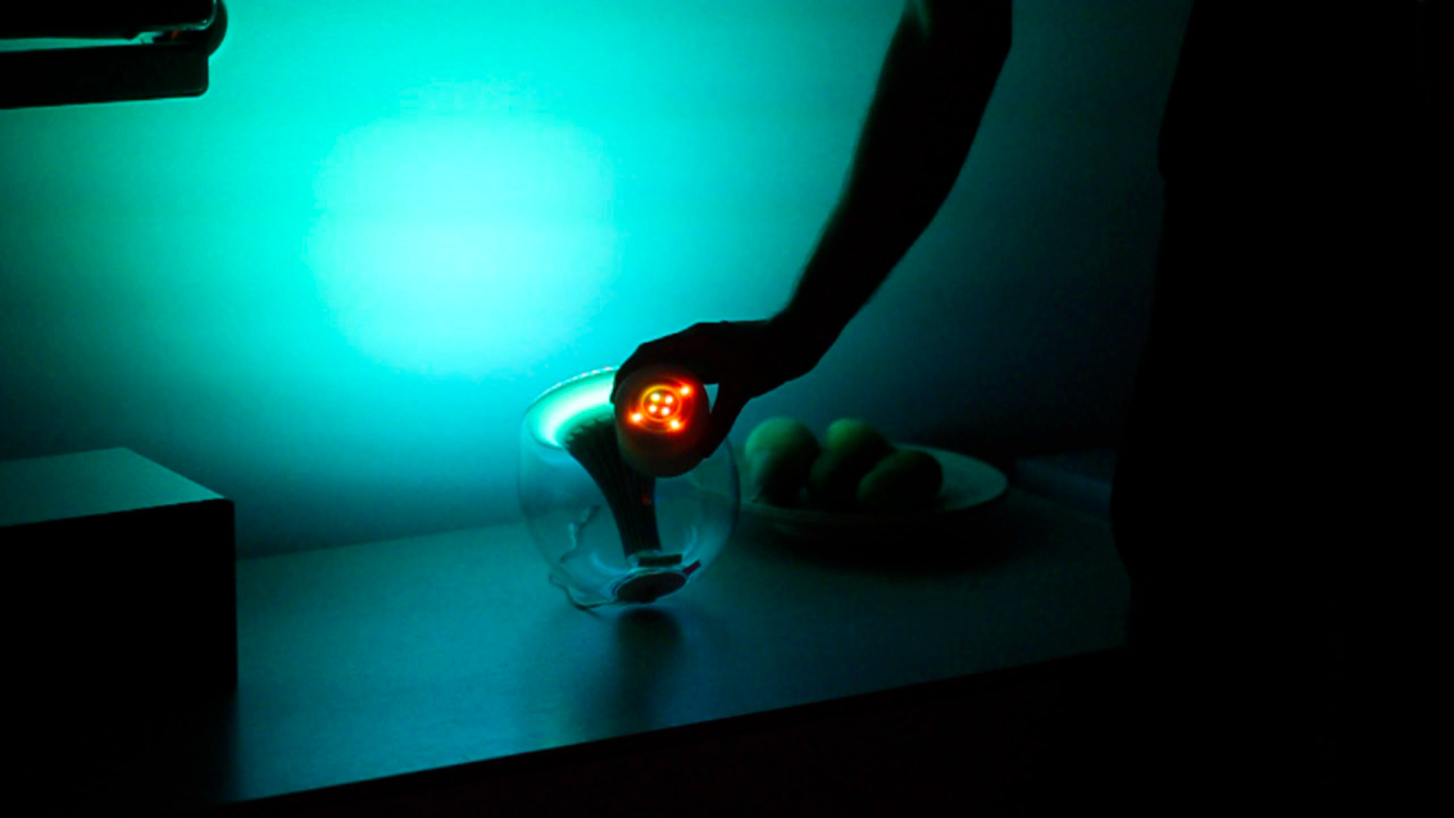
\includegraphics[width=300px]{LCscan}
\caption{Image showing the Connector scanning the lighting device.}
\label{LCscan}
\end{figure}

Philips created two lighting devices based on their LivingColors technology, that can be used to generate dynamic coloured lighting. Figure \ref{LCscan} shows the Connector object scanning a tag on the lighting device. These lighting devices accept a stream of RGB values and use the information to generate a sequence of coloured lighting. Using the media type descriptions introduced above, we can describe a lighting device as follows: 

\begin{minted}{turtle}
LightingDevice rdf:type SmartObject .
LightingDevice acceptsMediaType RGBValues .
LightingDevice rendersMediaAs Lighting .
\end{minted}

In the scenario there exists a permanent semantic connection between the two lighting devices. This means that when dynamic lighting is generated on one device, the same lighting will be displayed on the other device.

%The Bonding Device accepts dynamic lighting information in the form of a stream of RGB values. What makes this scenario interesting is that the mobile device itself is not capable of transmitting these RGB values, but the Sound/Light KP (a virtual device in the smart space) is. The Sound/Light KP acts as a semantic transformer, converting the music stream generated by the mobile device into the RGB values required by the Bonding Device. From the user's point of view, the only \textit{required} connection is that between the mobile device and the Bonding Device, while the smart space takes care of the rest.



\section{Implementation}
\label{D2Implementation}

%In this section we describe implementation details of how the concepts of the theory are modelled

\begin{figure}
\centerline{
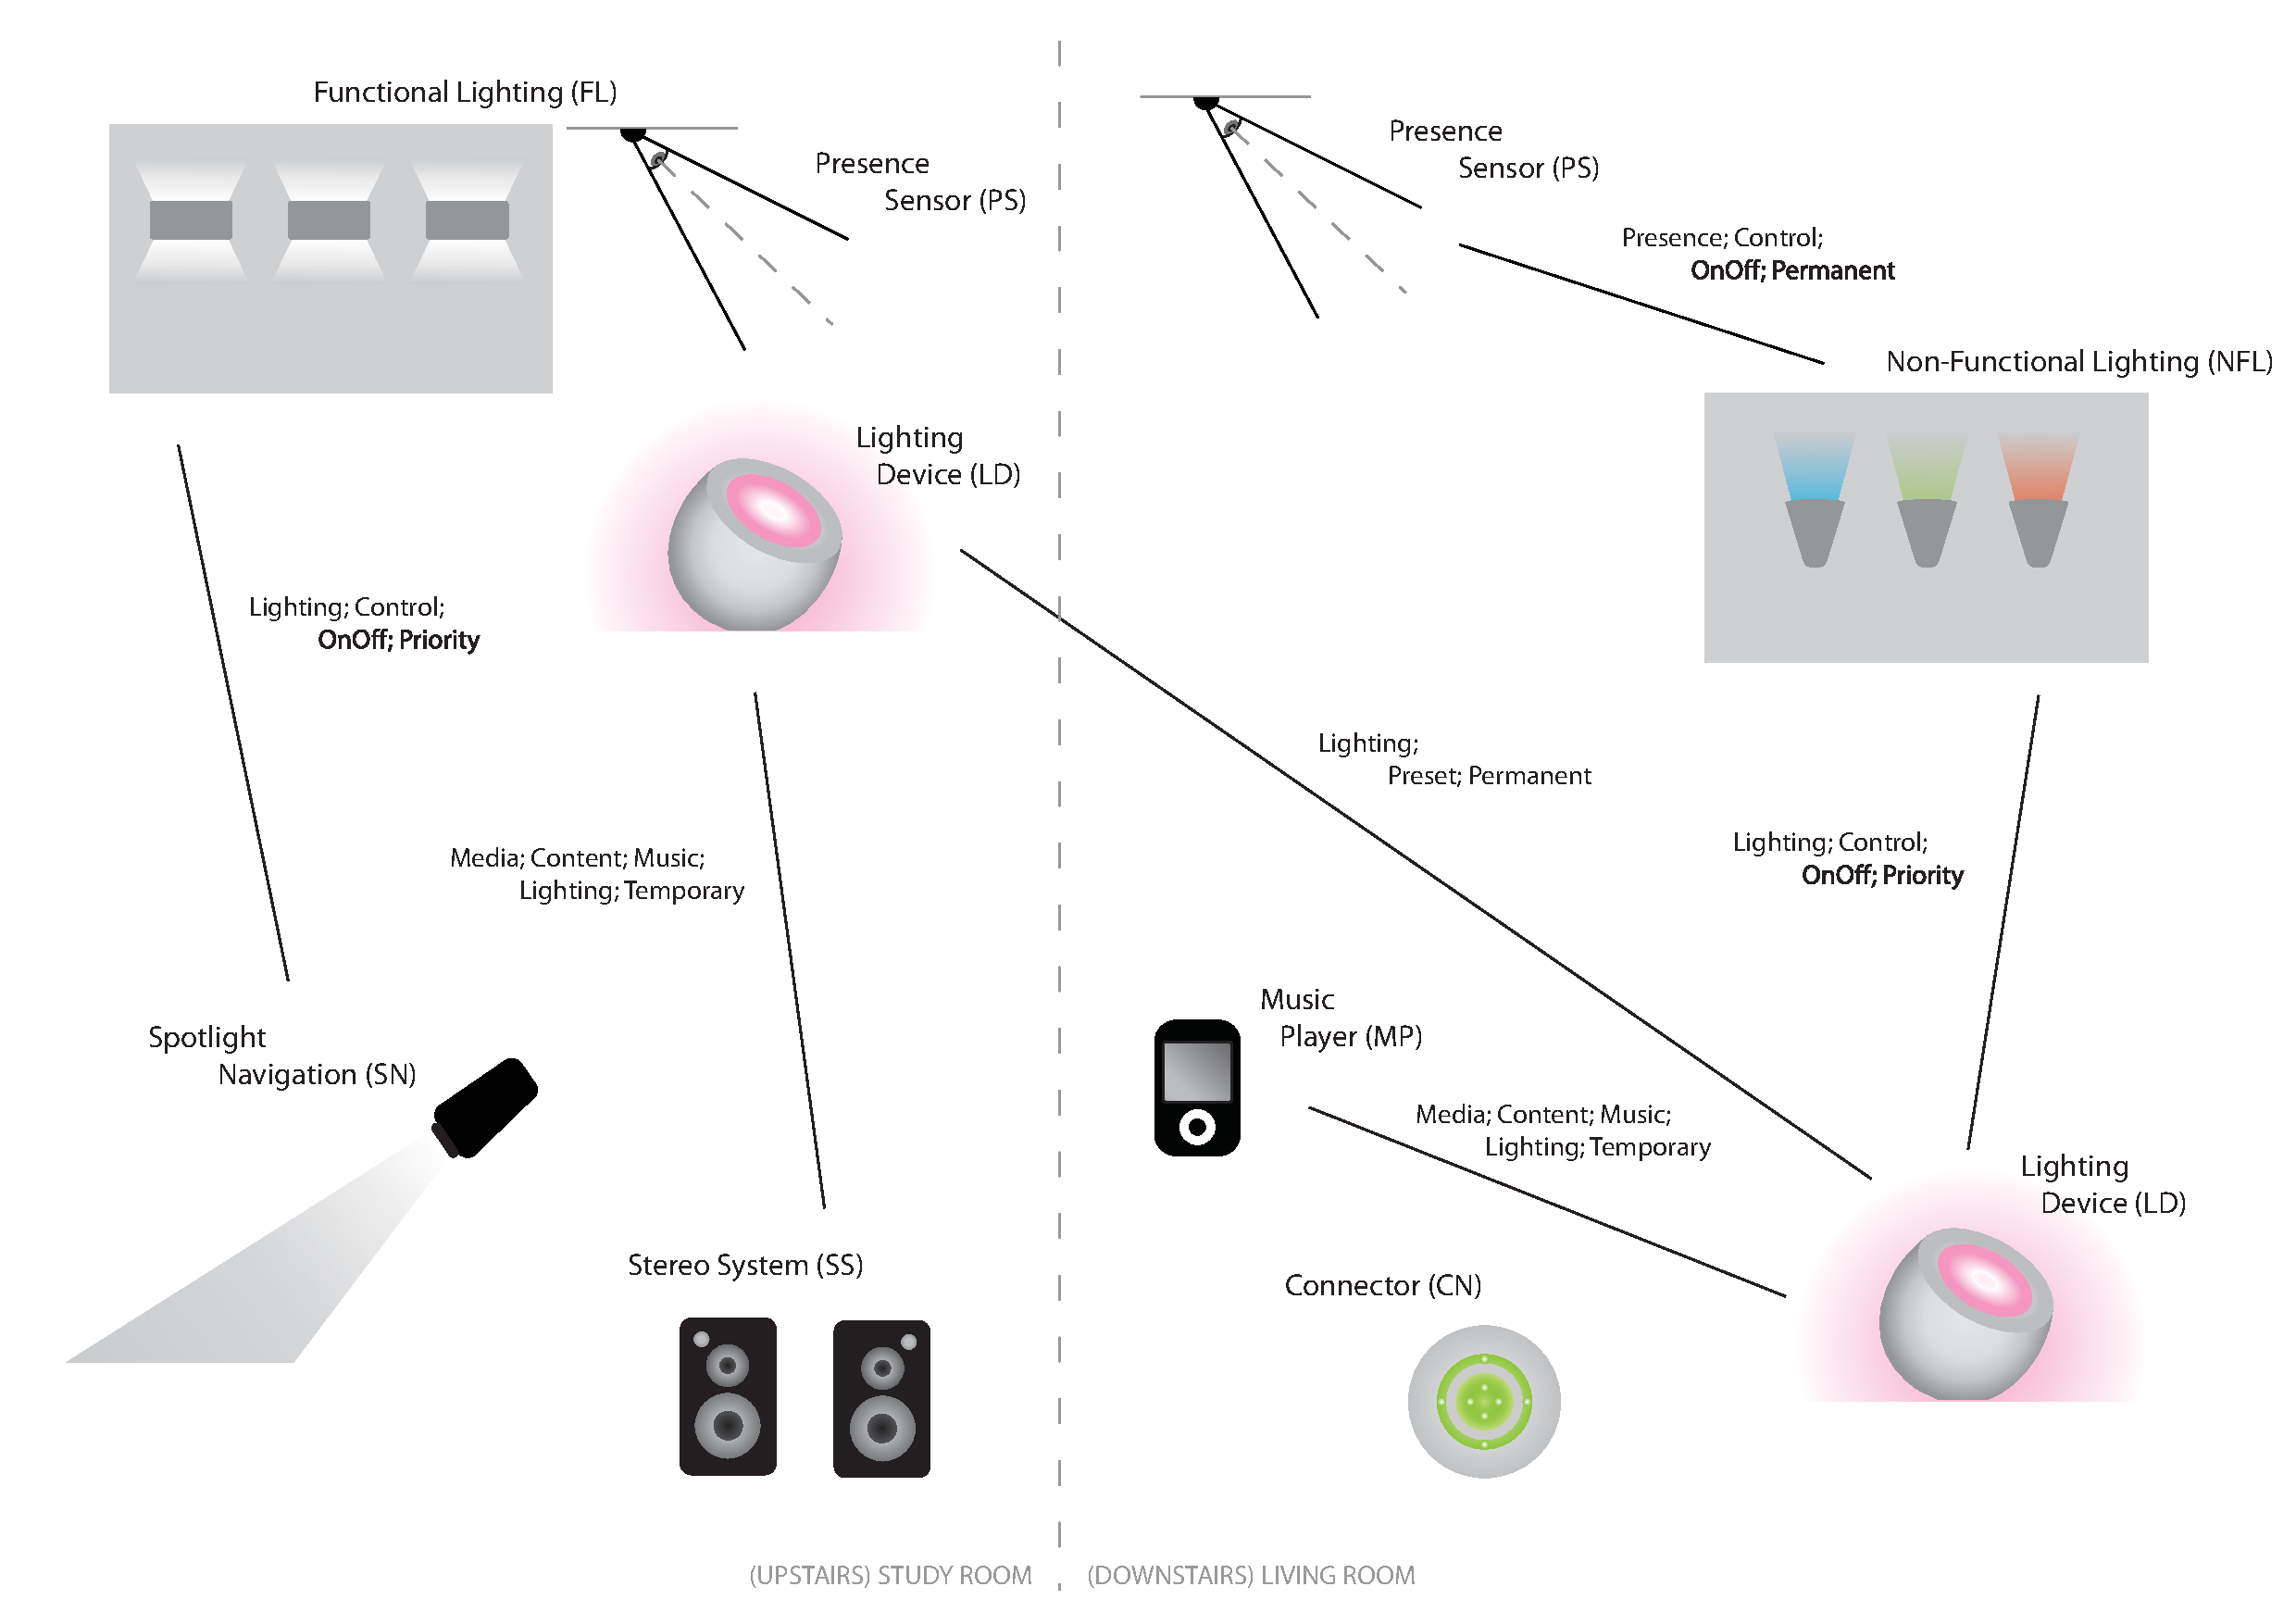
\includegraphics[width=\paperwidth-40mm]{pilotSetup}}
\caption{The devices and their connections as used in the system}
\label{pilotSetup}
\end{figure}

Figure \ref{pilotSetup} shows a brief overview of the different parts of the system. The experiment took place in two rooms, the study and the living room of the Experience Lab on the High Tech Campus in Eindhoven. During the pilot, users interacted with various automated and interactive appliances and devices defined as smart objects. There exist several semantic connections between the smart objects, for example the media-content connection between the phone and the lighting device, and the lighting-control connection between the lighting device and the non-functional lighting. Some of these connections can be explicitly interacted with through two interaction devices: a Spotlight Navigation device placed in the study of the pilot setup upstairs, or a Connector device placed in the living room of the pilot setup downstairs. 

% The Spotlight Navigation device is a mobile device containing a pico projector that visualises connection possibilities between devices in the environment. By using direct pointing gestures with the device in the user's hand, users can intuitively explore and manipulate the virtual network connections as if they are part of the user's real world environment. The Connector device follows a tangible interaction approach, enabling users to physically select devices in their environment and directly view and manipulate the connections in a simple, universal way. It is a hand-held device that identifies devices by scanning RFID tags that are located on the devices themselves. By holding the Connector on top of the tag, users can explore the connection possibilities that are visualised with lights on top of the Connector. After holding the device in the RFID field for a moment, the device-ID is locked and the other device to be connected can be selected in a similar fashion. With a push-to-click action a connection between two devices can be established. For removing an existing connection, the ring on the lower part of the device should be pulled until it clicks. 

 %A video of the Smart Home pilot is available online\footnote{}. (Not public)



In the Smart Home pilot, media content is shared among several smart objects in a smart home setting. Music can be shared between a mobile device, a stereo speaker set and a lighting device that can render the mood of the music with coloured lighting. The music experience is also shared remotely between friends living in separate homes through the lighting device. This light and music information is shared between the two lighting devices. Other lighting sources, like the smart functional lighting (FL, Figure \ref{pilotSetup}) and the smart wall wash lights (NFL, Figure \ref{pilotSetup}) are sensitive to user presence and the use of other lighting sources in the environment. The setup was built using the \ac{SOFIA} software platform as is described in Chapter \ref{SoftwareArchitecture}. A diagram showing the technical details of the Smart Home pilot is shown in Figure \ref{SmartHomePilotDiagram}. It gives an indication of the variety and complexity of the hardware platforms, operating systems and wireless protocols that were used.

%alternative is to use pdfpages, but textpos seem to work fine
% \newpage
% \thispagestyle{empty}
% \begin{textblock*}{\paperwidth-10mm}(10mm,10mm)
%         \begin{figure}
% 		\centering
% 		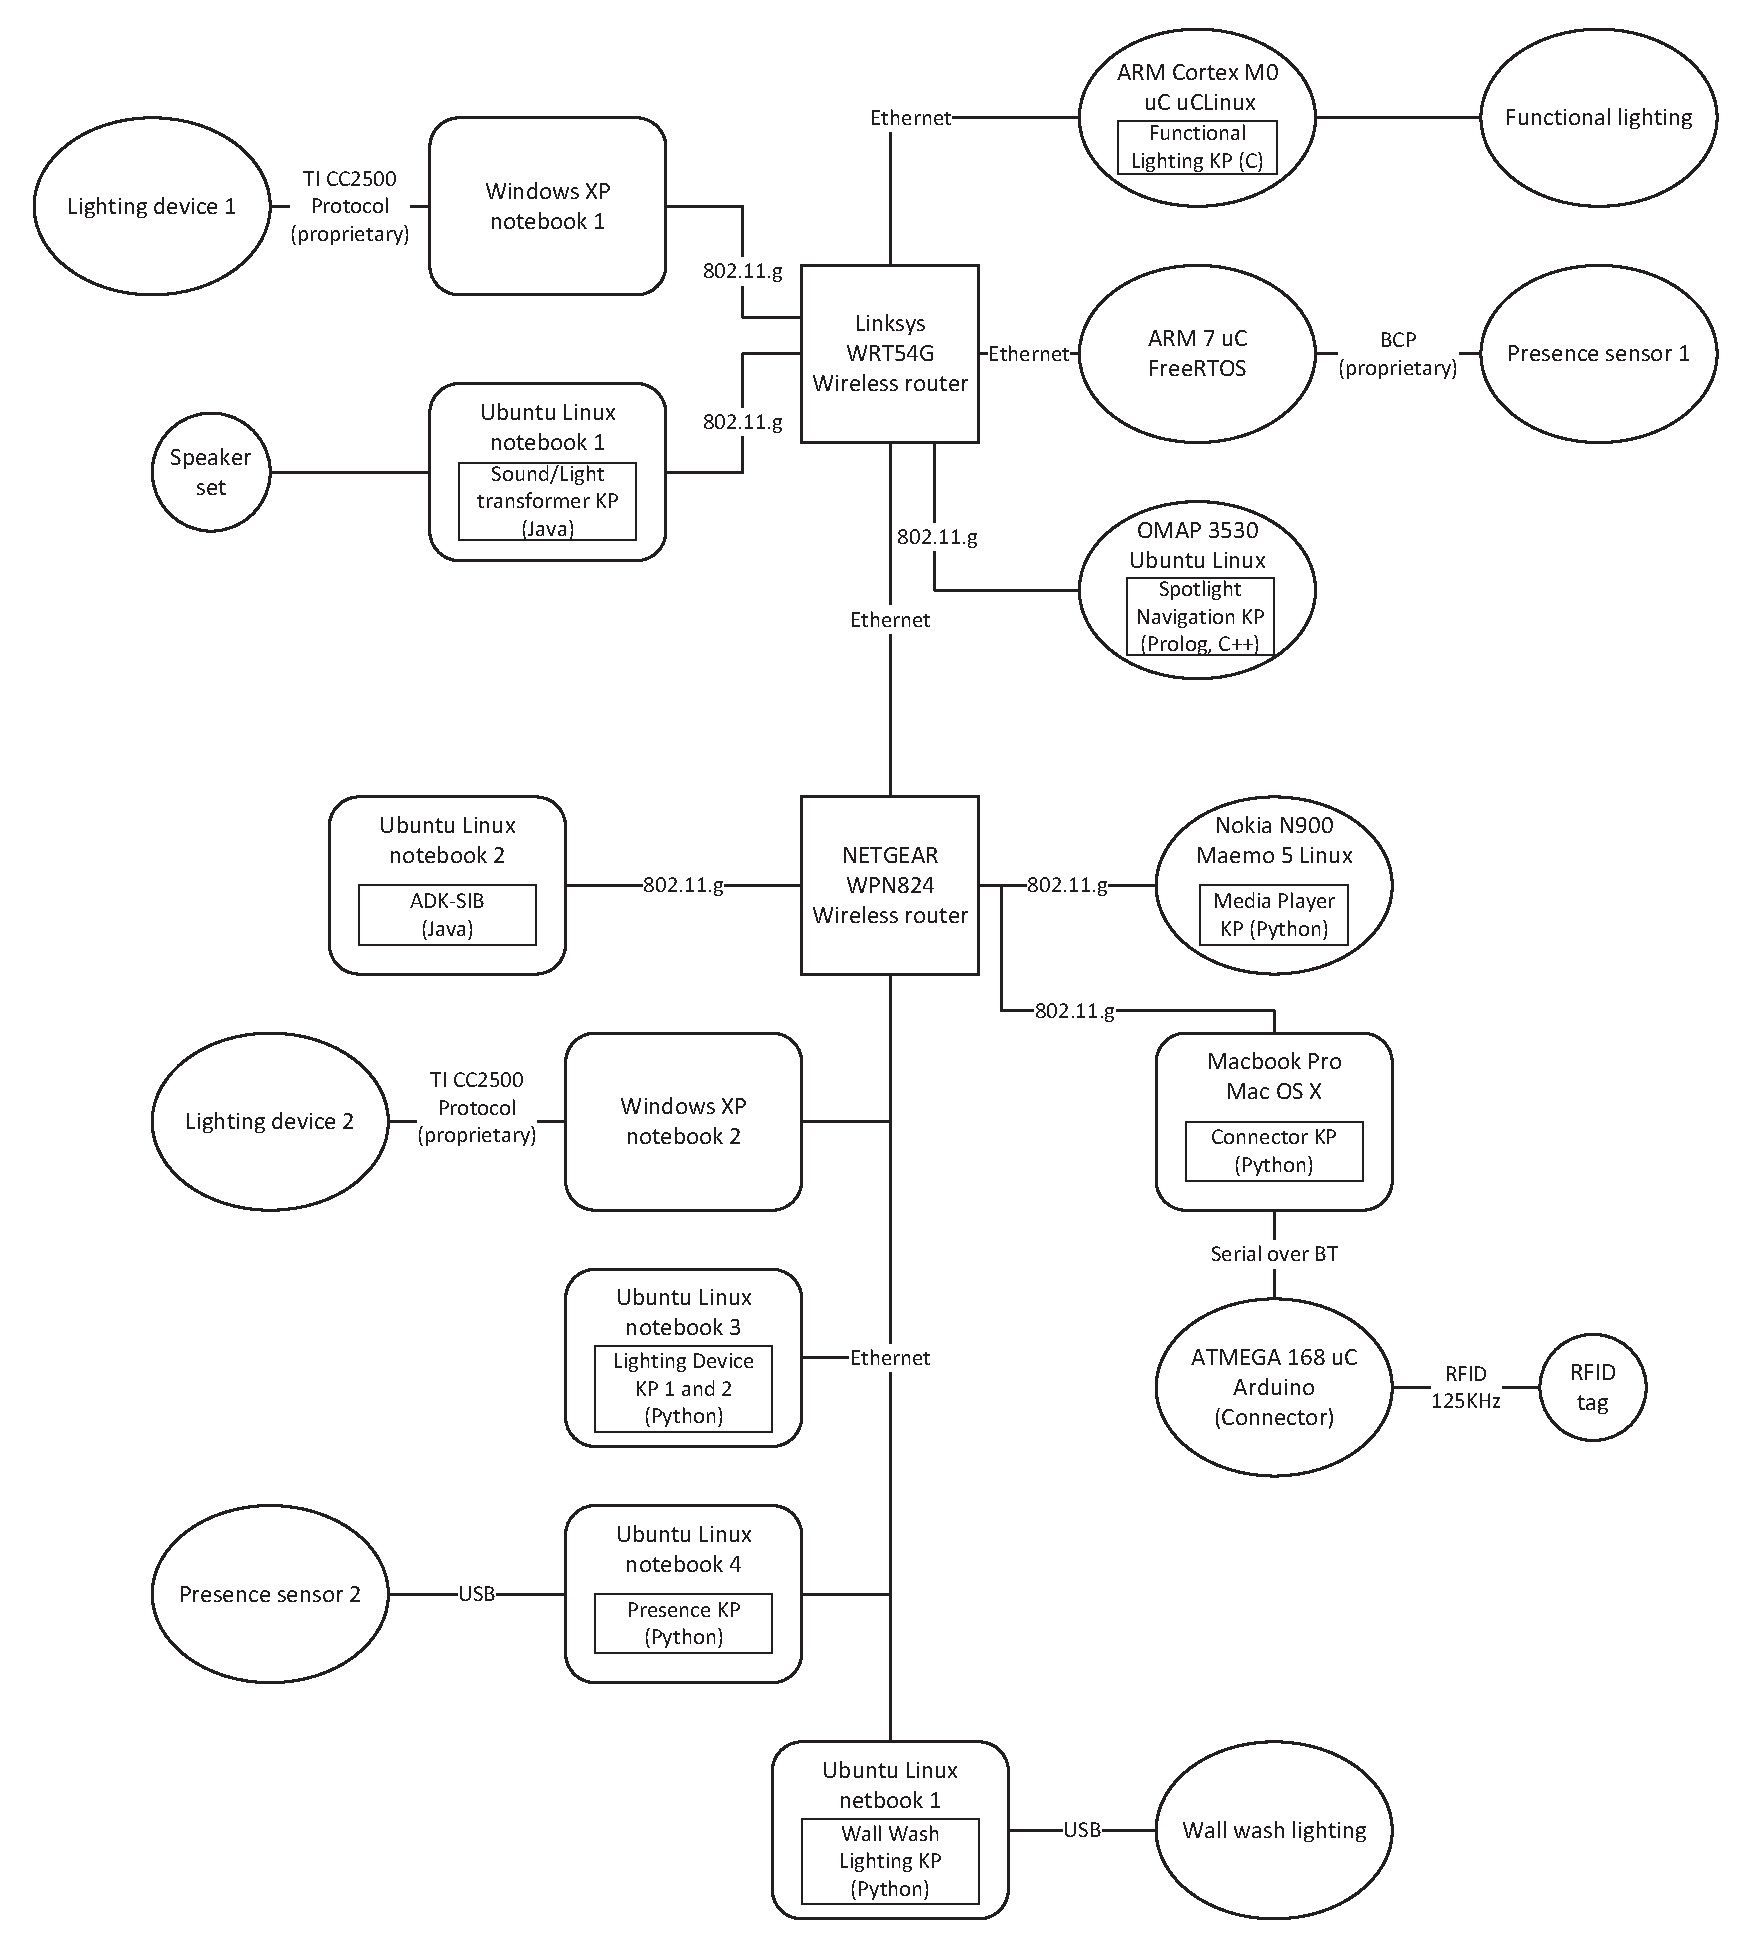
\includegraphics[width=\paperwidth-20mm]{SmartHomePilotDiagram}
% 		\caption{Technical details of the Smart Home pilot}
% 		\label{SmartHomePilotDiagram}
% 		\end{figure}
% \end{textblock*}
% \mbox{}\newpage


\begin{figure}
		\centerline{
		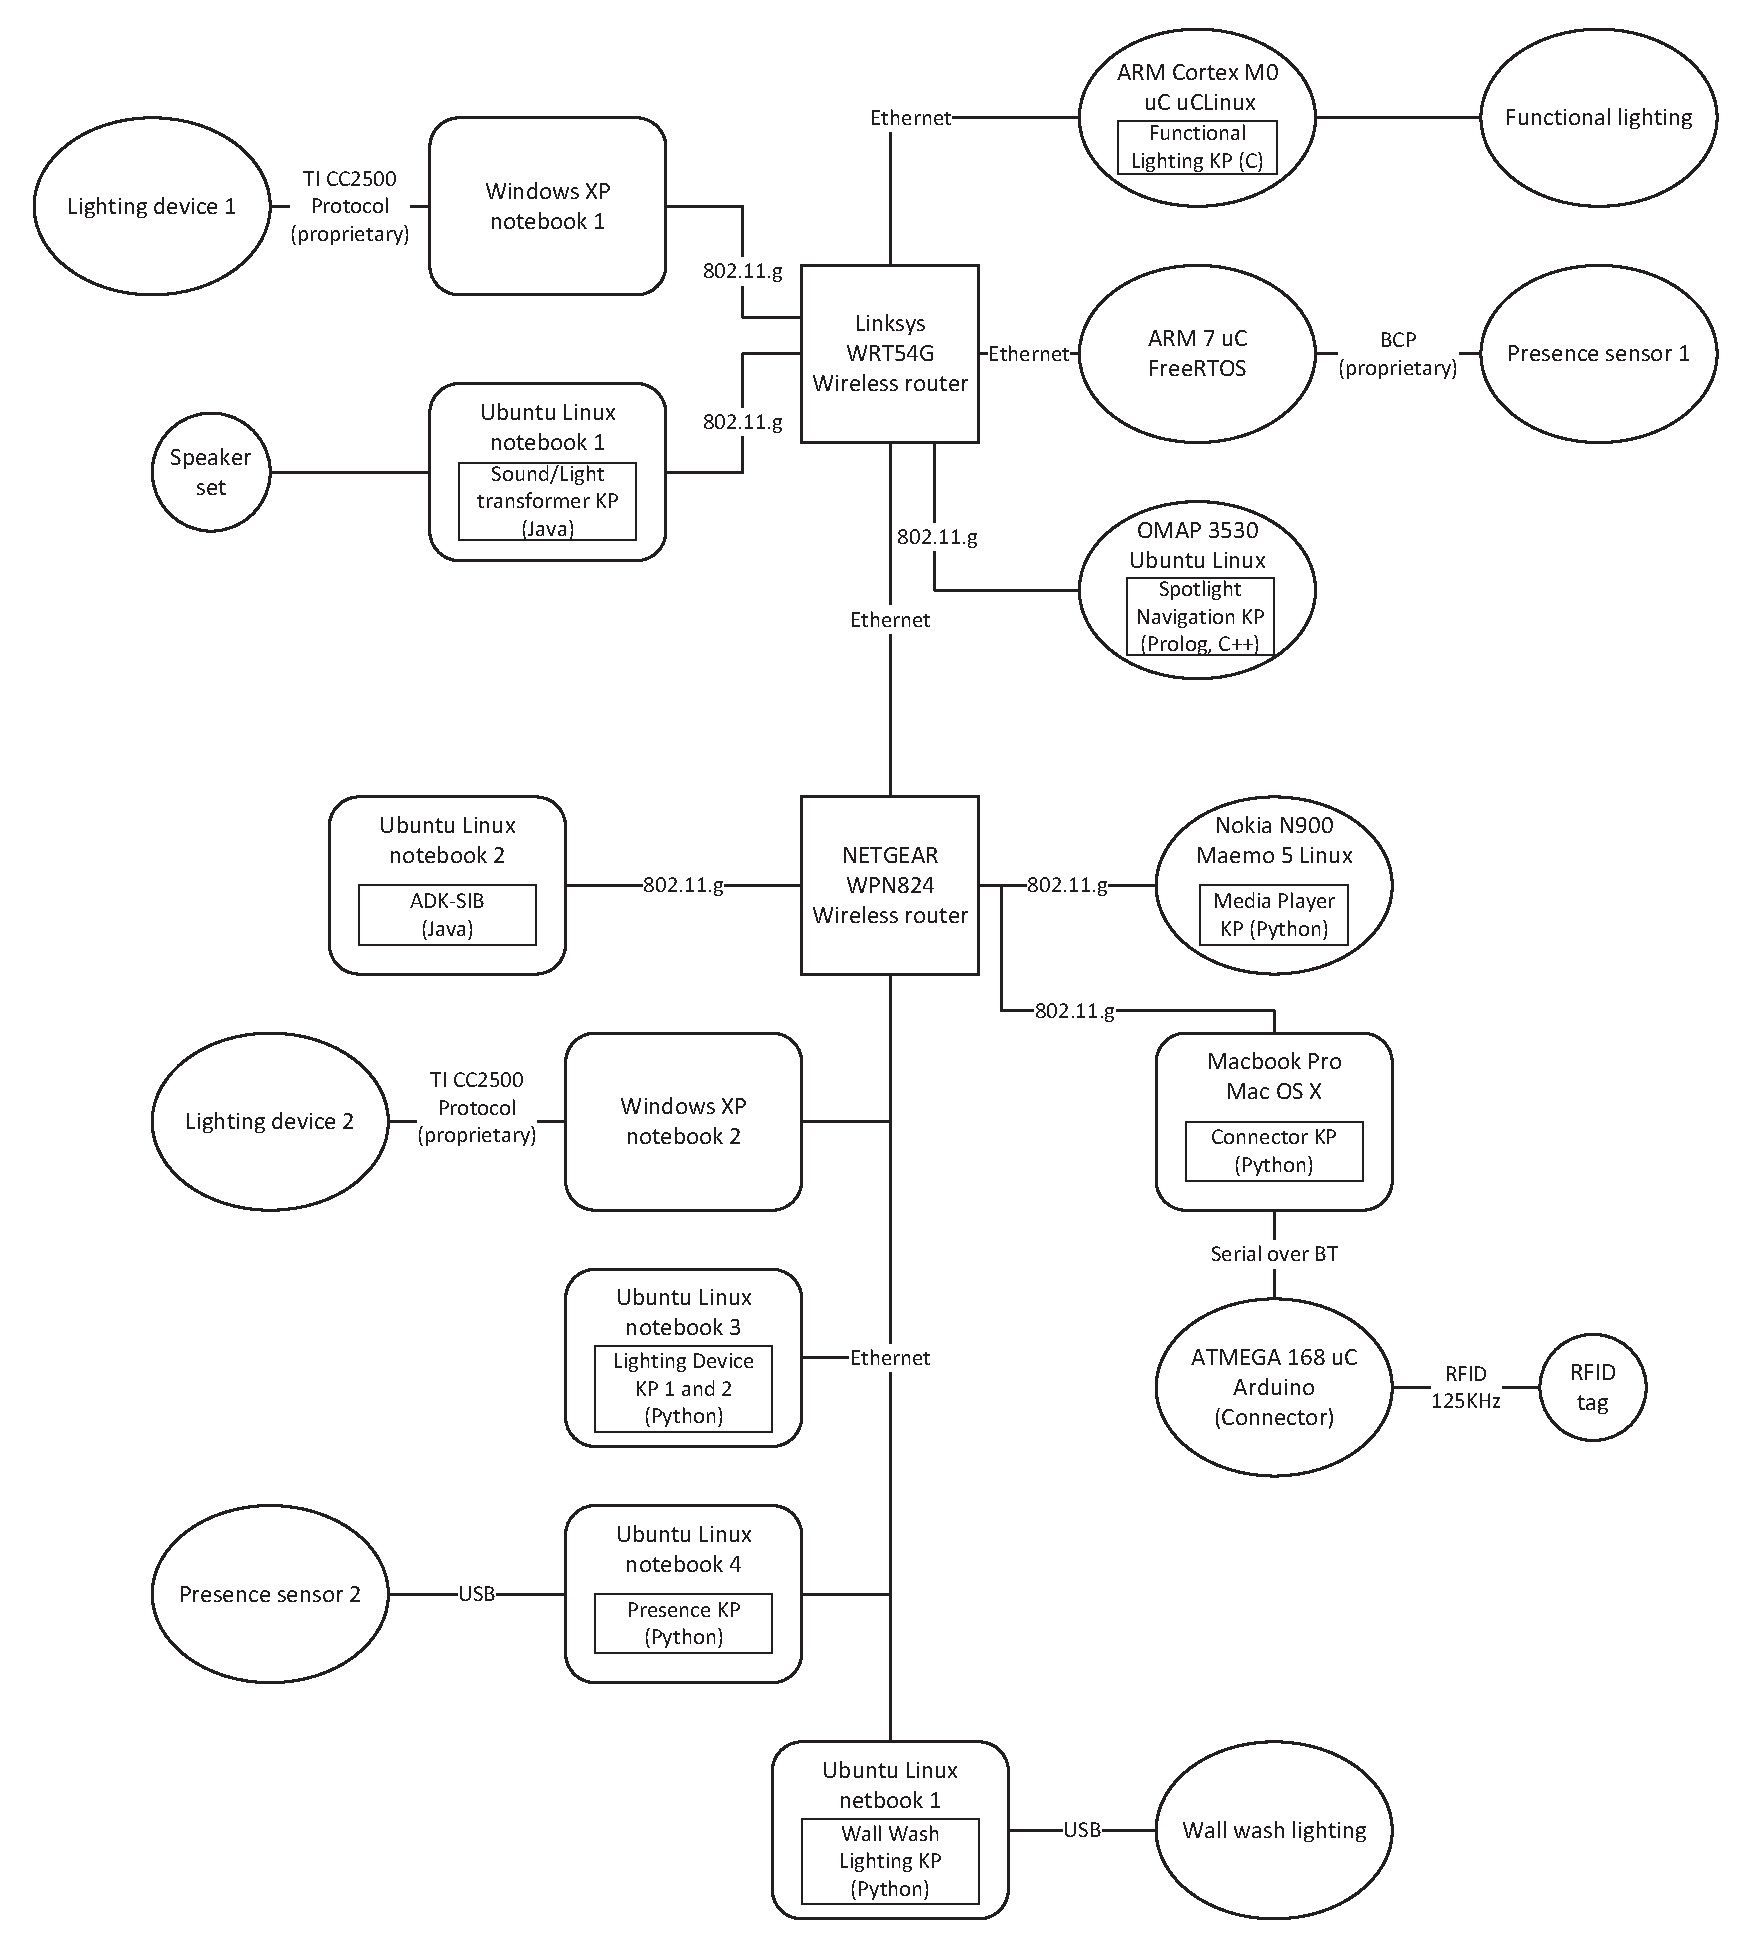
\includegraphics[width=\paperwidth-40mm]{SmartHomePilotDiagram}}
		\caption{Technical details of the Smart Home pilot}
		\label{SmartHomePilotDiagram}
\end{figure}



% from deliverable
% During the pilot, users experience a smart space with various automated and interactive appliances and devices (smart objects). The appliances in the smart space are interoperable, sensitive to changes in their environment and exchange information with one another. There are several explicit and implicit relations between the smart objects, of which some can be explicitly viewed or manipulated with the Spotlight Navigation device or the Connector device, available in two different locations.
% In the Smart Home Pilot, media content is shared among several devices in a smart home setting. Music can be shared between a mobile device, a stereo speaker set (connected to the smart space through a Sound/Light KP) and a Family Bonding Device that as one of its capabilities can render the mood of the music with coloured lighting. The music experience is also shared remotely between friends living in separate homes through the Bonding Device. This light and music information is shared between the two lighting devices. Other lighting sources, like the smart functional lighting from NXP and the smart wall wash lights (TU/e-SAN) are sensitive to user presence and the use of other lighting sources in the environment.

% We illustrate our implementation of semantic transformers by means of a use case scenario, where the semantic transformers were introduced as part of a smart home pilot (as defined in the SOFIA project). 

%In the Smart Home pilot, media content is shared among several devices in a smart home setting. Music can be shared between a mobile device, a stereo speaker set  and a lighting device that can render the mood of the music with coloured lighting.

\subsection{ADK-SIB}
\label{adk-sib}
In this iteration a new \ac{SIB} developed within the \ac{SOFIA} project was used, called the ADK-SIB. The ADK-SIB is a Jena-based\marginpar{The Jena framework was first mentioned in Section \ref{Jena}.} \ac{SIB} written in Java and runs on the \ac{OSGi} framework. Some modifications were made to the standard ADK-SIB provided by the \ac{SOFIA} project, such as reasoning support added with the TopBraid SPIN API 1.2.0\footnote{http://topbraid.org/spin/api/}. To run the \ac{SIB} from the \ac{OSGi} prompt, the \ac{SIB} and TCP/IP gateway is started separately as services:

\begin{minted}{console}
sspace create -sib -name=test
sspace create -gw -name=testgw -type=TCP/IP -idSib=1
sspace start -sib -id=1
sspace start -gw -id=1
\end{minted}

The \ac{SIB} and gateway are linked with one another through their IDs, enabling multiple \acp{SIB} and gateways to run on the same machine. \ac{OSGi} services have to be deployed as plugins from within the Eclipse development framework.

Reasoning on information contained within the \ac{SIB} was performed using \ac{SPIN}\footnote{http://www.spinrdf.org}. With SPIN, rules are expressed in \ac{SPARQL}, the W3C recommended \ac{RDF} query language, which allows for the creation of new individuals using CONSTRUCT queries. \ac{OWL} inferences for the \ac{OWL} 2 \ac{RL} profile were executed by using \ac{SPIN} rules\footnote{ http://topbraid.org/spin/owlrl-all}. OWL 2 RL is a syntactic subset of OWL 2 that is amenable to implementation using rule-based technologies. According to the OWL 2 RL W3C page\footnote{http://www.w3.org/TR/owl2-profiles/\#OWL\_2\_RL} the OWL 2 RL profile is aimed at applications that require scalable reasoning without sacrificing too much expressive power. 

\subsection{Semantic matching of media types}
\label{SemanticMatching}

A semantic transformer, called the Sound/Light KP, accepts a music stream as input and generates a stream of RGB values based on an analysis of the music stream. The Sound/Light KP is described as follows:

\begin{minted}{turtle}
SoundLightKP rdf:type SemanticTransformer .
SoundLightKP acceptsMediaType Audio .
SoundLightKP transmitsMediaType RGBValues .
SoundLightKP  hasIdentification id4321 .
id4321 ofIDType IPAddress .
id4321 idValue "192.168.1.4:1234" .
\end{minted}

The stream of RGB values is sent via a separate TCP/IP connection, so the lighting device needs to know whether the source device is capable of communicating via TCP/IP. Since smart objects in the smart space can be identified using their IP address and port number, we can use the identification information to infer a \texttt{communicatesByTCPIP} data property that can be read by the Bonding Device. To relate the \texttt{SmartObject} directly to the \texttt{IDType}, we use an \ac{OWL} 2 property chain:

\begin{quote}
hasIdentification~\ensuremath{\circ}~ofIDType~\ensuremath{\sqsubseteq}~hasIDType\footnote{The concatenation of two relations $R$ and $S$ is expressible by $R \circ S $, while $ R \sqsubseteq S$ indicates that $R$ is a subset of $S$ }
\end{quote}

\noindent We then infer the \texttt{communicatesByTCPIP} data property by specifying a \texttt{TCPIPObject} subclass:

\begin{minted}{turtle}
Class: TCPIPObject

    EquivalentTo:
        hasIDType value IPAddress 
        communicatesbyTCPIP value true

    SubClassOf:
        SmartObject 
\end{minted}

In order to determine the media source for the lighting device, we first need to  perform semantic matching of the media type descriptions. We first define \texttt{isAccepted\-MediaTypeOf} as the inverse property of \texttt{acceptsMediaType}, and then define the following property chain:

\begin{quote}
transmitsMediaType~\ensuremath{\circ}~isAcceptedMediaTypeOf~\ensuremath{\sqsubseteq}~convertsMediaType
\end{quote}

\begin{figure}
\centering
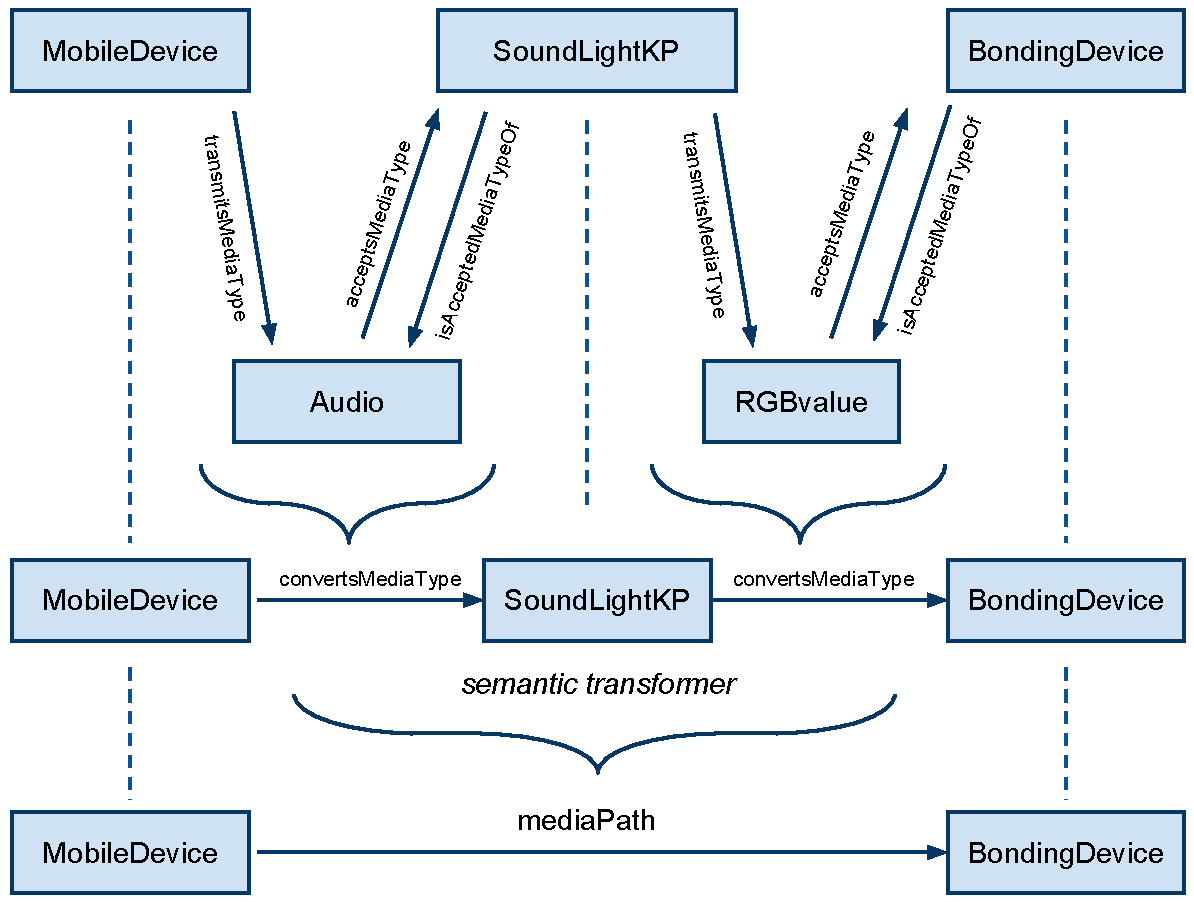
\includegraphics[width=250px]{SemanticTransformers}
\caption{Inferring the media path}
\label{mediapath}
\end{figure}

This allows us to match media types between smart objects. We can then infer a \textit{media path} between the mobile device and the Bonding Device with the Sound/Light KP acting as a semantic transformer using another property chain:

\begin{quote}
convertsMediaType~\ensuremath{\circ}~convertsMediaType~\ensuremath{\sqsubseteq}~mediaPath
\end{quote}

\noindent To then determine the media source itself we use \ac{SWRL}\footnote{http://www.w3.org/Submission/SWRL/}, as the expressivity of \ac{OWL} does not allow for inferring the media source if there are more than one \texttt{convertsMediaType} relationship linked to the lighting device:\\


\texttt{\scriptsize
convertsMediaType(?x1,?x2)~\ensuremath{\wedge}~convertsMediaType(?x2,?x3)~\ensuremath{\Rightarrow}~mediaSource(?x3, ?x2)}\\

The media source is the semantic transformer, \texttt{?x2}, while the media path is between the two smart objects, \texttt{?x1} and \texttt{?x3}. The \texttt{mediaSource} relationship is thus inferred from the smart object to the semantic transformer. We can also infer whether a device is a semantic transformer or not using:\marginpar{This \ac{SWRL} implementation was later replaced using another Semantic Web technology called SPIN, detailed in Chapter \ref{OntologyEngineering}.}


\begin{minted}{turtle}
Class: SemanticTransformer

    EquivalentTo:
        (canAcceptMediaTypeFrom some SmartObject) and
        (convertsMediaType some SmartObject)

    SubClassOf:
        SmartObject
\end{minted}


The end result is that the lighting device responds to the mobile device's media events (based on the Semantic Connections \texttt{connectedTo} relationship), but uses the Sound/Light KP as a media source for generating dynamic lighting. The \texttt{connectedTo} relationship between the mobile device and the lighting device should only be possible if a media path exists between the two devices. Figure \ref{mediapath} illustrates the entire process of inferring the media path from the original media type definitions.
%end africon

If the reasoner infers a media path between two smart objects, it does not mean that they are automatically connected -- it means that a connection is possible. The user can view this connection possibility using either the Connector device or the Spotlight Navigation device, and then establish the connection if necessary.

\subsection{Device states}

Interaction events (Chapter \ref{EventModelling}) cause device state changes. Most of the developers that worked on the Smart Home Pilot preferred to describe their smart objects in terms of the device states, and also shared these device states with other smart objects using the SIB. The current state of the smart object was defined using the \texttt{sofia:isInState} property:

\begin{minted}{turtle}
	conante:spotlight1 sofia:isInState "projecting" .
	sofia:nflKP1234 sofia:isInState "lightingON" .
	sofia:nflKP5678 sofia:isInState "lightingOFF" .
	sofia:presenceKP1234 sofia:isInState "Away" .
	sofia:presenceKP5678 sofia:isInState "Present" .
\end{minted}

These smart objects were all simple two-state devices, where the device state was indicated using a text field. Note that \texttt{conante:spotlight1} used the absence of \texttt{sofia:isInState} property to indicate that it was not projecting. This statement is valid with a \ac{CWA}, the presumption that that what is not currently known to be true, is false. The programmer that created this state description is well versed in the Prolog programming language, which makes the \ac{CWA}. \ac{OWL}, on the other hand, operates under the \ac{OWA}. With \ac{OWA}, we assume that new information can become available at any time, so that we cannot draw conclusions based on the assumption that all information is already available \cite{Allemang2011}. We can use the ontology to restrict how state descriptions are reported, forcing smart objects to report their current state at all times.\marginpar{The \ac{OWA} is also discussed in Section \ref{CardinalityRestrictions}.}




\section{Evaluation}
\label{D2Evaluation}
A number of issues were identified during a user study of the Smart Home pilot, described in more detail in \cite{VanderVlist2012a}. In the Smart Home pilot there were two locations connected via a permanent semantic connection between the lighting devices. What if Sofia were to play a song in her room --- will the same song play back at the home of Mark and Dries? If this is the case, we clearly need to introduce a notion of directionality in the semantic connections. This issue is addressed in Design Iteration III in the next chapter.

Early performance tests indicated that the Pellet reasoning engine with \ac{SWRL} rules proved to be a performance bottleneck in the system. For example, Pellet took about 3 seconds to infer 107 statements.\marginpar{In one instance, a \ac{SWRL} rule took up to 28 seconds to execute.} TopBraid Composer's TopSPIN reasoning engine supports \ac{SPIN} rules and \ac{OWL} 2, so it was tested as a possible alternative. The TopSPIN engine with OWL 2 RL/RDF Rules took less than a second to infer 10 491 triples. By using a hashmap to store our inferred triples, we were able to improve performance even further. Some of the inferred triples were redundant inferences -- by using a hashmap we were able to reduce the number of inferred triples on startup from 10 491 to 5 122, eliminating redundant triples.

A more formal performance evaluation as well as a user evaluation of the ontology, both of which were performed on the work done in this iteration, is discussed in Chapter \ref{Evaluation}.

% - Evaluation: 
% 	- How to define dim level, InUse state. 
% 	- If song 1 is playing in location 1, and song 2 is in location 2, which gets preference? -> directionality needed
% 	- Early SIB performance measurements (22/03/11, also GDocs)
% 	- Comparing SPIN+Pellet to SPIN+OWL2RL/RDF Rules:
% 		- Pellet takes 3 seconds to realize 107 elements
% 		- OWL2RL/RDF Rules takes less than a second to infer 11 361 triples
% 		- OWL2R/RDF Rules performance further improved by storing inferred triples in hashmap (see implementation). Also reduced number of inferred triples on startup form 10 491 to 5 122
		
		
\section{Discussion \& Conclusion}
\label{D2Discussion}
%\subsection{Implementation issues}

Modelling constraints in the ontology is done using \emph{restrictions}.  When modelling concepts in an \ac{OWL} ontology, restrictions are defined either as part of \texttt{rdfs:subClassOf} or as part of \texttt{owl:e\-quiv\-a\-lent\-Class}. There is a subtle difference, and it has to do with \emph{necessary and sufficient conditions}.

When we have necessary and sufficient conditions (also known as \emph{if and only if} and denoted as $ \equiv $, $ \leftrightarrow $ or $ \Leftrightarrow $), the \texttt{owl:e\-quiv\-a\-lent\-Class} restriction (denoted as $ \equiv $) is used. When we only have necessary conditions, the \texttt{rdfs:subClassOf} restriction (denoted as $ \sqsubseteq $) is used. \emph{Necessary and sufficient} means that the restriction is sufficiently constrained that only individuals belonging to that class will be classified as such.\footnote{In the Prot\'eg\'e ontology editor these are also called \emph{defined classes}.} An example is shown in Section \ref{SemanticMatching}. \marginpar{An \ac{OWL} reasoner follows a bottom-up approach, where new information is inferred from asserted facts, compared to a theorem prover that starts from its goal.}



% Idempotency is the property of being able to perform the same action twice or more times in sequence, and end up with the same result as if the action was performed once. In the triple store, defining a smart object or interaction primitive is idempotent as long as the definition  doesn't change on the triple-level. The idempotency of interaction events depends on whether a new timestamp is used when inserting the event into the triple store.
% 
% 
% ==TODO Idempotence
% Idempotence is the property of being able to perform the same action twice or more times in sequence, and end up with the same result as if it was performed once. As an example, consider the different HTTP methods:
% 
% \begin{itemize}
% 	\item PUT - uploads a representation of a specified resource
% 	\item DELETE - deletes the specified resource
% 	\item POST - can either update an existing resource or create a new resource
% \end{itemize}
% 
% PUT and DELETE are idempotent, while POST is not. In our case, creating a new interaction event is not idempotent, but inserting the same triple twice is. In the triple store, defining a smart object or interaction primitive is idempotent as long as the definition  does not change on the triple level. The idempotence of interaction events depends on whether a new timestamp is used when inserting the event into the triple store.



The ontology supports the description of interaction data generated by interaction devices and sensors. Additionally, it shows that an interaction primitive may trigger an interaction event or a state change that may need to be specified in more detail by a more application-specific ontology. That is to say, this ontology may also be used to perform semantic mapping from the interaction data to user goals and/or available services \cite{Niezen2010}. Any additional information related to the smart object may be added by extending the schema defined in the Semantic Interaction Ontology. 

Another advantage of the ontology described in this section is that opens up the way to context-based interaction device reconfiguration. For example, if a Context Monitor application recognises a situation where the \texttt{PhoneRockerSwitch} should no longer control the volume, but adjust the level of lighting instead, the triple could be modified accordingly. Just such a simple change would implement a behaviour that adapts to the situation.

Context-dependent functionality changes of a control may not necessarily be a desirable feature. It should however be noted that we only consider context-dependent meaning change with generic interaction primitives, that in itself do not have a specific, function related meaning (and might already being used for different functions, like the rocker switch in the example). Additionally, the re-mapping is only considered for those interaction elements with compatible transformational properties, e.g. the rocker switch may only be mapped to other \texttt{AdjustLevel} transformations, and not to \texttt{Start/Stop}. The specified range measures are used to control the re-mapping between a interaction primitive and an interaction event, in a similar way that the input and output domains of \cite{MacKinlay1990} are used to control the expressiveness between an input device and its application parameter. 

The question then becomes how to inform the user of the remapping in a user-friendly way. In the next chapter we consider the different types of feedback that can be used. Besides automatic context-dependent functionality changes of controls, we especially consider user-initiated re-mapping of controls. By enabling users to make associations, or semantic connections \cite{VanderVlist2010} between devices or interaction elements and devices, users can express their intentions in terms of mapping controls between devices \cite{Niezen2010}. 

% While most of the issues discussed in this paper also applies to user interaction in general, 
% the way in which interaction events and interaction primitives are distributed between multiple devices makes our work very applicable to ubiquitous computing environments. Semantic mapping between interaction primitives and interaction events on different devices is also supported.
% 
% The use of interaction primitives to model the essential elements of user interaction is currently being implemented by various project partners, and up until now seem promising. A thorough evaluation and validation is part of our next steps, as well as integration of the introduced concepts into the SOFIA core ontology or application- or domain-specific ontologies.
%end africon

% Spotlight Navigation and the Connector are two alternative user interface approaches to configuring ubiquitous computing infrastructure. Although we cannot directly compare the mental models elicited during the user experiment, which would have asked for a more controlled setting (e.g. having the same setup and having an equal number of participants for both treatments), we did make some interesting observations.

% The most striking difference between the way users described the setup was the perception of the users that the Connector was part (if not the central part) of the system, while the Spotlight Navigation was often considered outside of the system. We hypothesise that this is due to the different roles that the Spotlight Navigation and the Connector have in the interaction with the connections. The Connector is used to conceptually ``carry'' the content between the two devices and in itself represents the relation between these two artefacts. The Spotlight Navigation is, in contrast, perceived as a ``remote control'' that visualises the connections in physical space. This might lead the users to conclude that the projected lines are the connections, directly between the devices, and leave the Spotlight Navigation itself outside of this network.

%begin S3E
Judging from the experience of implementing the semantic transformers, the approach of using them to solve interoperability problems appears promising. Using the Semantic Media Ontology, we were able to define a smart object in terms of the media types it accepts and transmits. Based on these descriptions, semantic transformers can be used to transform media types in order to enable information exchange between devices that would normally not be able to communicate. With only a minimal set of device capabilities described, the system is able to perform self-configuration using semantic reasoning.
%end S3E

%begin africon
Even though the Semantic Interaction Ontology describes parts of a \texttt{SmartObject}, it does not fully describe all the properties and capabilities of the smart object. It only describes its in\-ter\-ac\-tion-related properties. Particularly it defines the \texttt{SmartObject} interaction primitives and means of identification. In the next chapter, while describing the next iteration, we will focus on expanding the possibilities of describing a device's functionality and capabilities.


